% Overleaf's default compiler looks for a file literally named main.tex.
% The actual paper (per the original file-structure spec) lives in paper.tex;
% this thin wrapper just pulls it in so the project compiles out of the box
% without needing to change Overleaf's "Main document" project setting.
\documentclass[conference]{IEEEtran}

\usepackage{amsmath}
\usepackage{amssymb}
\usepackage{graphicx}
\usepackage{booktabs}
\usepackage{multirow}
\usepackage{tikz}
\usetikzlibrary{shapes.geometric, arrows.meta, positioning, fit, backgrounds}
\usepackage{url}
\usepackage{cite}
\usepackage[hidelinks]{hyperref}
\usepackage{array}
\usepackage{subcaption}

\graphicspath{{figures/}{images/}}

\begin{document}

\title{Cost Belongs in the Constraint, Not the Objective:\\ A Held-Out Evaluation of Multi-Criteria Model Selection\\ for Retail Demand Forecasting}

\author{

\IEEEauthorblockN{Ranjith Kumar N}
\IEEEauthorblockA{
Department of Computer Science and Engineering\\
PES University\\
Bengaluru, Karnataka, India\\
PES1UG23CS474
}

\and

\IEEEauthorblockN{Pooja Ammalajeri}
\IEEEauthorblockA{
Department of Computer Science and Engineering\\
PES University\\
Bengaluru, Karnataka, India\\
PES1UG23AM203
}

\and

\IEEEauthorblockN{Gayathri M}
\IEEEauthorblockA{
Department of Computer Science and Engineering\\
PES University\\
Bengaluru, Karnataka, India\\
PES1UG23CS217
}

\and

\IEEEauthorblockN{Preetham Kumar S}
\IEEEauthorblockA{
Department of Computer Science and Engineering\\
PES University\\
Bengaluru, Karnataka, India\\
PES1UG23AM213
}

\thanks{Project Guide: Dr. Jyothi R, Department of Computer Science and Engineering, PES University, Bengaluru, Karnataka, India.}

}

\maketitle

\begin{abstract}
Retail demand forecasting is complicated by heterogeneous data sources, irregular seasonality, intermittent demand for slow-moving items, and the reluctance of business stakeholders to act on predictions they cannot interpret. This paper presents the design and implementation of an end-to-end retail demand forecasting system that trains nineteen forecasting models spanning statistical, machine learning, deep learning, and intermittent-demand families in parallel on a single uploaded dataset, and automatically selects the best-performing model using a robust, multi-criteria composite score rather than a single error metric. The system is implemented as a FastAPI backend and a React single-page frontend, accepts CSV, Excel, and JSON files describing arbitrary time-indexed retail, energy, or transactional data, and performs automated column detection, gap filling, outlier capping, and optional exogenous-feature integration (price and promotional indicators) for the models capable of using them. Beyond numerical accuracy, the system addresses the interpretability gap directly: native feature-importance scores from the tree-based models are surfaced to the user, and a retrieval-augmented large language model layer, grounded in a curated corpus of retail domain knowledge and in the deterministic metrics computed by the pipeline, generates natural-language explanations, a conversational question-answering interface, and a proactive business insights report. Particular engineering attention is given to trustworthiness: forecast uncertainty intervals are derived from each model's own historical cross-validation error rather than an arbitrary fixed percentage, and the language model is explicitly constrained to never contradict the deterministic trend and volatility labels the system itself computes. The system is evaluated on a real retail transaction dataset aggregated to a daily sales series; twelve of the nineteen registered models complete successfully within the automatically inferred data-frequency tier, with the k-nearest-neighbor regressor selected as the best model under the composite score despite extreme gradient boosting achieving a marginally lower root-mean-squared error, illustrating the practical difference between single-metric and multi-criteria model selection. The results and architecture indicate that a broad, automatically-adjudicated model ensemble combined with a grounded natural-language explanation layer is a practical and extensible approach to trustworthy retail forecasting.
\end{abstract}

\begin{IEEEkeywords}
demand forecasting, retail analytics, time series analysis, machine learning, deep learning, ensemble model selection, explainable artificial intelligence, retrieval-augmented generation
\end{IEEEkeywords}


\section{Introduction}
\label{sec:introduction}

\subsection{Background}
Accurate demand forecasting underlies nearly every operational decision a retail organization makes: inventory replenishment, staffing, pricing, promotional planning, and supply-chain coordination all depend on a credible estimate of how much of a given product will sell over a future horizon~\cite{fildes2022retail}. Retail sales series are shaped simultaneously by long-run trend, weekly and annual seasonality, promotional events, price changes, and idiosyncratic noise, and different products within the same organization can exhibit qualitatively different demand patterns, from smooth, high-volume staples to sparse, intermittent demand for slow-moving or newly introduced items~\cite{croston1972}. No single forecasting technique performs best across this diversity of patterns, a conclusion repeatedly reinforced by large-scale forecasting competitions such as the M4 and M5 competitions~\cite{makridakis2020m4,makridakis2022m5}.

\subsection{Business Motivation}
For small and mid-sized retailers in particular, the practical obstacle is rarely the absence of a suitable algorithm in the academic literature; it is the absence of a system that (i) works across heterogeneous, often messy uploaded datasets without bespoke data-engineering effort, (ii) selects an appropriate model automatically rather than requiring in-house data-science expertise, and (iii) produces an output that a non-technical manager can trust and act upon. A forecast that is numerically accurate but delivered as an opaque number, with no explanation of why a particular model was chosen or how confident the system is, is of limited practical value to a retail operations team.

\subsection{Challenges in Retail Forecasting}
Three challenges recur throughout this problem space. First, \emph{heterogeneity}: uploaded datasets vary in file format, column naming convention, date format, sampling frequency, and completeness, and a forecasting pipeline intended for general use must detect and normalize all of these automatically. Second, \emph{model selection under uncertainty}: because no model dominates across all series, a credible system must train a diverse set of candidates and adjudicate among them using an evaluation procedure that is robust to a single badly-fit outlier model distorting the comparison. Third, \emph{intermittent and small-sample regimes}: many retail items sell too infrequently, or a dataset is too short, for computationally expensive models such as deep neural networks to be trained reliably, and a well-designed system should recognize this rather than train models likely to overfit or fail silently.

\subsection{Machine Learning and Deep Learning Approaches}
Statistical time-series methods such as ARIMA and Holt-Winters exponential smoothing~\cite{boxjenkins1970,winters1960holtwinters} remain strong baselines, particularly on short series, and modern additive-regression tools such as Prophet~\cite{taylor2018prophet} extend this family with automatic seasonality and holiday-effect modeling. Tree-based machine learning models, most notably random forests~\cite{breiman2001randomforest} and gradient-boosted trees~\cite{chen2016xgboost}, have proven competitive on tabular, feature-engineered representations of time series, while recurrent architectures such as LSTM and GRU networks~\cite{hochreiter1997lstm,cho2014gru}, convolutional sequence models such as temporal convolutional networks~\cite{bai2018tcn}, and attention-based transformer architectures~\cite{vaswani2017attention} have extended the state of the art on longer, richer series, at the cost of requiring substantially more training data to avoid overfitting~\cite{lim2021survey}.

\subsection{The Need for Explainable AI}
A parallel and increasingly important line of work addresses the interpretability of forecasting and machine learning systems more generally. Post-hoc explanation techniques such as SHAP~\cite{lundberg2017shap} and LIME~\cite{ribeiro2016lime} have become common tools for exposing feature-level contributions to individual predictions, and the broader emergence of instruction-following large language models~\cite{brown2020gpt3,devlin2019bert} has opened a complementary avenue: rather than only exposing numerical attributions, a system can generate a natural-language explanation of its own output. When such a language model is grounded in retrieved domain knowledge and in the system's own deterministic computations, using a retrieval-augmented generation architecture~\cite{lewis2020rag}, the risk of the explanation contradicting or fabricating facts about the underlying forecast can be substantially reduced. This is the approach adopted in the system described in this paper.

\subsection{Research Motivation}
The motivation for this work is therefore not to propose a new forecasting algorithm, but to design and implement a complete, end-to-end system that (i) is dataset-agnostic across retail, transactional, and general time-series data; (ii) trains and fairly adjudicates a broad ensemble of nineteen models spanning statistical, machine learning, deep learning, and intermittent-demand families; (iii) degrades gracefully rather than failing when a dataset is too small or a candidate model is unsuitable; and (iv) closes the interpretability gap using a combination of native feature-importance scores and a grounded, retrieval-augmented language model layer, rather than treating the forecast as an opaque endpoint.

\subsection{Contributions}
The contributions of this paper are summarized as follows.
\begin{itemize}
    \item A unified orchestration layer that trains nineteen forecasting models (seven statistical, four classical machine learning, seven deep learning, and one intermittent-demand model) concurrently on an arbitrary uploaded time series, using an adaptive walk-forward cross-validation scheme whose fold count scales with the available data.
    \item A robust, multi-criteria model-selection score that normalizes root-mean-squared error, mean absolute error, mean absolute percentage error, forecast stability, computation time, and coefficient of determination using a Tukey-fence-based robust scale, preventing a single catastrophically mis-fit model from distorting the ranking of the remaining candidates.
    \item A frequency-aware gating mechanism that withholds deep learning models from datasets below an empirically justified minimum row count, communicating this decision explicitly to the end user rather than training and reporting on an unreliable model.
    \item Integration of real exogenous features (price and promotional indicators), when present in the uploaded dataset, into the gradient boosting, random forest, and seasonal autoregressive models, with an explicit and conservative policy for extending these features into the unobserved forecast horizon.
    \item A retrieval-augmented, large-language-model explanation layer, grounded simultaneously in a curated retail-domain knowledge base and in the pipeline's own deterministic metrics, that provides a conversational question-answering interface and a structured business insights report, with explicit prompt-level constraints preventing the language model from contradicting the system's own computed labels.
    \item An empirical evaluation of the complete pipeline on a real retail transaction dataset, reporting accuracy, computation time, and the practical divergence between single-metric and multi-criteria model selection.
\end{itemize}

\subsection{Paper Organization}
The remainder of this paper is organized as follows. Section~\ref{sec:literature} reviews related work in retail and time-series forecasting, machine learning and deep learning approaches, and explainable artificial intelligence. Section~\ref{sec:problem} states the problem addressed and the corresponding research gap. Section~\ref{sec:proposed} describes the proposed system architecture and workflow. Section~\ref{sec:dataset} describes the dataset used for evaluation and the automated preprocessing pipeline. Section~\ref{sec:methodology} details every implemented forecasting model, including governing equations. Section~\ref{sec:xai} describes the explainability layer. Section~\ref{sec:architecture} presents the system architecture diagrams. Section~\ref{sec:experimental} describes the experimental setup. Section~\ref{sec:results} reports quantitative results. Section~\ref{sec:discussion} interprets these results. Section~\ref{sec:future} outlines future work, and Section~\ref{sec:conclusion} concludes the paper.

\section{Literature Review}
\label{sec:literature}

\subsection{Retail and Demand Forecasting}
Retail forecasting has a long history as an applied field distinct from generic time-series analysis, owing to domain-specific complications such as promotions, price elasticity, new-product introduction, and stockouts~\cite{fildes2022retail,ord2017principles}. Large-scale empirical competitions have played a disproportionate role in establishing what actually works in practice. The M4 competition~\cite{makridakis2020m4} compared 61 forecasting methods across 100{,}000 series and found that combination methods and, later, hybrid statistical-machine-learning approaches outperformed both pure statistical and pure machine learning methods in isolation. The subsequent M5 competition~\cite{makridakis2022m5} specifically targeted retail sales data from a large retailer and confirmed that gradient-boosted tree methods were highly competitive on real retail series, while also highlighting the difficulty of forecasting intermittent, low-volume items accurately. These findings directly motivate the multi-model, automatically-adjudicated design adopted in this paper, rather than committing to a single model family a priori.

\subsection{Statistical Time-Series Forecasting}
The Box-Jenkins ARIMA methodology~\cite{boxjenkins1970} and its seasonal extension SARIMA remain foundational statistical approaches, modeling a series as a function of its own past values and past forecast errors after appropriate differencing. Exponential smoothing methods, including the Holt-Winters method~\cite{winters1960holtwinters}, model level, trend, and seasonal components multiplicatively or additively and remain highly competitive baselines, particularly for shorter series where more complex models are prone to overfitting~\cite{hyndman2018forecasting,makridakis1998forecasting}. More recently, additive regression frameworks such as Prophet~\cite{taylor2018prophet} were designed explicitly for business forecasting at scale, decomposing a series into trend, multiple seasonalities, and holiday effects, and are notable for degrading gracefully on noisy or irregular business data.

\subsection{Machine Learning for Time Series}
Framing time-series forecasting as a supervised regression problem over engineered lag, rolling-statistic, and calendar features allows conventional machine learning regressors to be applied directly. Random forests~\cite{breiman2001randomforest} and gradient-boosted trees, particularly the XGBoost implementation~\cite{chen2016xgboost}, have become standard strong baselines in this framing and were prominent among top-performing methods in the M5 competition~\cite{makridakis2022m5}. Instance-based methods such as $k$-nearest-neighbor regression~\cite{cover1967knn} and kernel methods such as support vector regression~\cite{cortes1995svm} are comparatively lightweight alternatives that can be competitive on smaller datasets where tree ensembles or neural networks have insufficient data to realize their capacity advantage.

\subsection{Deep Learning for Time Series}
Recurrent neural architectures, especially the long short-term memory (LSTM) network~\cite{hochreiter1997lstm,gers2000forget} and the gated recurrent unit (GRU)~\cite{cho2014gru}, were designed to model long-range temporal dependence while mitigating the vanishing-gradient problem of simple recurrent networks. Convolutional alternatives, including the temporal convolutional network~\cite{bai2018tcn}, achieve comparable or superior performance on some sequence-modeling benchmarks with better parallelization. Attention-based transformer architectures~\cite{vaswani2017attention} have subsequently been adapted specifically for long-sequence time-series forecasting, for example in the Informer architecture~\cite{zhou2021informer}, while specialized forecasting-native deep architectures such as DeepAR~\cite{salinas2020deepar} and N-BEATS~\cite{oreshkin2020nbeats} target probabilistic and interpretable forecasting respectively. A consistent finding across this literature, and a central empirical justification for the frequency-aware gating mechanism introduced in this paper, is that deep sequence models require substantially more training observations than statistical or tree-based methods to generalize reliably~\cite{lim2021survey}; when applied to short series they are prone to memorizing noise rather than learning genuine temporal structure.

\subsection{Hybrid and Meta-Learning Approaches}
A separate line of work combines statistical and machine-learning components directly, for example residual-correction hybrids in which a statistical model captures linear trend and seasonality while a neural network models the remaining nonlinear residual~\cite{zhang2003hybrid}. Meta-learning approaches for retail forecasting~\cite{ma2021metalearning} instead learn to select or weight among candidate models based on series characteristics. The system described in this paper adopts a related but simpler and more transparent strategy: every candidate model is always trained and evaluated identically via walk-forward cross-validation, and selection is performed by an explicit, auditable composite scoring rule rather than a learned meta-model, prioritizing transparency over marginal accuracy gains.

\subsection{Intermittent Demand Forecasting}
Standard forecasting methods perform poorly on sparse, intermittent demand series in which a large fraction of periods have zero recorded demand, a pattern common for slow-moving retail items and spare parts. Croston's method~\cite{croston1972} addresses this by separately smoothing the non-zero demand size and the inter-demand interval and forecasting their ratio as a constant rate. The Syntetos-Boylan approximation~\cite{syntetos2005sba} subsequently identified and corrected a systematic positive bias in Croston's original estimator, and is the variant adopted in this paper's implementation.

\subsection{Evaluation Methodology for Time Series}
Correctly evaluating time-series models requires respecting temporal ordering; naive random train-test splits leak future information into the training set and inflate reported accuracy. Walk-forward, expanding-window cross-validation is the accepted alternative~\cite{bergmeir2012cv}, and the number of folds used should reasonably reflect the amount of data available, since too few folds increases the risk that a model appears best due to chance performance on a single split~\cite{januschowski2020criteria}. Broader reviews of forecasting practice~\cite{petropoulos2022forecasting} additionally emphasize that a single point accuracy metric such as root-mean-squared error is an incomplete criterion for model selection in practice, since it does not capture computational cost, forecast stability, or the risk profile of a badly-calibrated model; this observation directly motivates the multi-criteria composite scoring approach described in Section~\ref{sec:methodology}.

\subsection{Explainable AI and Retrieval-Augmented Generation}
Post-hoc, model-agnostic explanation techniques such as SHAP~\cite{lundberg2017shap}, grounded in cooperative game-theoretic Shapley values, and LIME~\cite{ribeiro2016lime}, based on local surrogate modeling, are widely used to attribute a model's prediction to its input features. Tree-based models additionally expose a native, computationally inexpensive impurity- or gain-based feature-importance measure as a byproduct of training, which the system described in this paper surfaces directly for its gradient boosting and random forest models rather than computing a separate post-hoc attribution.

Independently, the emergence of large, instruction-following language models~\cite{brown2020gpt3,devlin2019bert} has introduced natural-language generation as a complementary explanation modality: rather than exposing numerical attributions alone, a system can narrate its reasoning in prose intelligible to a non-technical stakeholder. The central risk of this approach is hallucination, the generation of fluent but factually incorrect statements. Retrieval-augmented generation~\cite{lewis2020rag} mitigates this risk by conditioning language-model generation on retrieved, verifiable source documents rather than relying purely on the model's parametric knowledge. The explanation layer described in this paper applies this principle twice: qualitative business advice is grounded in a retrieved, curated retail-domain knowledge base, while all quantitative claims are grounded directly in the deterministic metrics computed by the forecasting pipeline itself, with explicit prompt-level instructions preventing the language model from re-deriving or contradicting labels the system has already computed.

\subsection{Positioning of This Work}
Relative to the reviewed literature, this paper does not propose a novel forecasting algorithm. Its contribution is architectural and systems-oriented: it integrates a broad, heterogeneous ensemble spanning all four model families discussed above behind a single automated pipeline, introduces an explicit and auditable robust multi-criteria selection rule in place of raw error-metric ranking, applies an empirically justified frequency-based gate to prevent unreliable deep-learning training on insufficient data, and couples the resulting forecasts to a retrieval-augmented natural-language explanation layer that is explicitly constrained to remain consistent with the system's own deterministic outputs.

\section{Problem Statement}
\label{sec:problem}

\subsection{Current Limitations}
Existing retail forecasting tooling accessible to non-specialist organizations typically exhibits one or more of the following limitations. First, many tools commit to a single model family, such as a single statistical method or a single machine learning regressor, and therefore perform inconsistently across the heterogeneous demand patterns present even within one retailer's catalogue, a pattern well documented by cross-method forecasting competitions~\cite{makridakis2020m4,makridakis2022m5}. Second, tools that do support multiple models frequently select among them using only a single point-accuracy metric, most commonly root-mean-squared error, which is sensitive to the scale of the series and does not account for computation cost, forecast stability, or the risk that one poorly calibrated model can distort a comparison against otherwise well-fitted competitors. Third, deep learning models are often applied uniformly regardless of dataset size, despite established evidence that they require substantially more observations than statistical or tree-based alternatives to generalize reliably~\cite{lim2021survey}; on short retail series this risks reporting an overfit model as though it were reliable. Fourth, and most consequential for adoption by non-technical stakeholders, the forecast is typically delivered as a bare number or chart with no accompanying explanation of model choice, uncertainty, or business implication, which limits the degree to which a retail manager can trust and act on the output.

\subsection{Research Gap}
The literature reviewed in Section~\ref{sec:literature} addresses these limitations largely in isolation: forecasting-competition research establishes which model families perform well on which data characteristics, evaluation-methodology research establishes how models should be validated, and explainable-AI research establishes how a trained model's behavior can be attributed or narrated. There is comparatively little published work describing a single, integrated system that combines a broad multi-family model ensemble, a robust and auditable multi-criteria selection rule, an explicit data-driven gate on which models are even attempted, and a language-model explanation layer that is architecturally constrained to remain factually consistent with the system's own deterministic computations. This integration gap, rather than any single algorithmic deficiency, is the specific research gap this paper addresses.

\subsection{Objectives}
The system described in this paper is designed to satisfy the following objectives.
\begin{enumerate}
    \item Accept an arbitrary time-indexed dataset in common tabular file formats and automatically identify the date column, the numeric target column, and any usable exogenous or grouping columns, without requiring the uploader to pre-process the file.
    \item Train a broad ensemble of forecasting models spanning statistical, classical machine learning, deep learning, and intermittent-demand families, evaluated identically via walk-forward cross-validation.
    \item Select the best-performing model using a composite criterion that is robust to a single outlier model and that reflects accuracy, stability, and computational cost jointly, rather than a single error metric alone.
    \item Withhold computationally expensive deep learning models from datasets below a data-driven minimum size, and communicate this decision transparently rather than silently degrading forecast quality.
    \item Incorporate real exogenous business features, specifically price and promotional indicators, into the subset of models capable of using them, when such columns are present in the uploaded dataset.
    \item Provide a natural-language explanation layer, grounded in retrieved domain knowledge and in the pipeline's own deterministic outputs, that answers user questions and produces a proactive business report without contradicting the system's own computed metrics or labels.
\end{enumerate}

\subsection{Expected Improvements}
Relative to a single-model or single-metric baseline, the proposed system is expected to improve robustness across heterogeneous retail series by virtue of its broad ensemble and adaptive model gating, to improve the trustworthiness of reported uncertainty by deriving forecast intervals from each model's own historical error rather than an arbitrary fixed percentage, and to improve the practical usability of the forecast for non-technical stakeholders through grounded natural-language explanation. These improvements are evaluated empirically in Sections~\ref{sec:experimental} and~\ref{sec:results}.

\section{Proposed System}
\label{sec:proposed}

\subsection{System Overview}
The proposed system is a full-stack web application comprising a Python FastAPI backend and a React single-page frontend, communicating over a REST HTTP API. The backend is organized into four logical layers: (i) an ingestion and preprocessing layer that accepts an uploaded file and produces a clean, gap-filled, outlier-capped time series together with any usable exogenous features; (ii) a model orchestration layer that trains the full ensemble of candidate forecasting models concurrently and computes a composite selection score; (iii) a persistence layer that caches forecast results and conversational state to disk, keyed by a client-generated session identifier, so that concurrent users or browser tabs do not overwrite one another's results and so that state survives a backend restart; and (iv) an explanation layer that generates natural-language narration of the forecast, grounded jointly in retrieved domain knowledge and in the pipeline's own deterministic metrics. Figure~\ref{fig:architecture} depicts the overall architecture.

\subsection{Workflow Overview}
From the end user's perspective, the workflow proceeds in four steps: (1) a dataset file is uploaded and the system responds with detected columns and suggested date, target, grouping, and exogenous-feature columns; (2) the user confirms or adjusts these column selections and a forecast horizon, and optionally selects a country code for holiday-effect modeling or a grouping value to forecast an individual product, store, or category; (3) the backend executes the full training and selection pipeline and returns the leaderboard of all attempted models together with the selected best model's forecast, uncertainty interval, and, where applicable, feature importance; and (4) the user may inspect a model-comparison chart, ask the conversational assistant questions about the result, or request a structured business insights report.

\subsection{Data Pipeline}
\label{subsec:data-pipeline}
The ingestion layer accepts CSV, Microsoft Excel (\texttt{.xlsx}/\texttt{.xlsm}), and JSON files. Column detection proceeds by a combination of dtype inspection, column-name keyword matching against curated vocabularies for date-like, target-like, grouping-like, price-like, and promotion-like columns, and, for date columns specifically, an ordered cascade of parsing strategies including native pandas inference, explicit format cycling, Unix-timestamp interpretation bounded to a plausible calendar-year range, and finally mixed-format parsing as a last resort. Once a date and target column are selected, the preprocessing pipeline (i) parses and coerces the target column to a numeric type, handling currency symbols, thousands separators, and both American and European decimal conventions; (ii) sets the date column as index and aggregates duplicate timestamps by summation, consistent with the assumption that duplicate timestamps represent multiple transactions on the same period; (iii) infers the dominant sampling frequency and reindexes to a complete, gap-free calendar at that frequency; (iv) fills newly introduced and pre-existing missing values through time-aware interpolation followed by forward- and backward-filling; (v) detects and Winsorizes outliers using an interquartile-range rule; and (vi) applies light rolling-median smoothing for high-frequency (sub-daily) series. If exogenous feature columns were selected, they are aligned to the same cleaned index using an aggregation rule appropriate to their type, price-like columns by mean and promotional-flag columns by maximum, and the resulting exogenous frame is retained separately from, but index-aligned with, the cleaned target series.

\subsection{Training Pipeline}
The orchestration layer submits every registered model to a shared thread pool and trains them concurrently, subject to a per-model timeout appropriate to its statistical, machine-learning, or deep-learning category. Each model is evaluated using walk-forward, expanding-window cross-validation, with the number of folds determined adaptively from the number of available observations, subject to a configured minimum and maximum. Deep learning models are withheld entirely, rather than trained and reported unreliably, when the series has fewer observations than an empirically justified minimum for its inferred sampling frequency, and this decision is surfaced explicitly to the end user together with its justification. When exogenous features are present, a request-scoped override of the model registry substitutes exogenous-aware variants of the gradient boosting, random forest, and seasonal autoregressive models, leaving the remaining models untouched, so that the shared orchestration logic itself does not need to be aware of which individual models accept additional arguments.

\subsection{Prediction Pipeline and Model Selection}
Once every model has completed training and cross-validation, or timed out or raised an exception, the selection layer first filters to models that both completed successfully and produced a numerically usable forecast, defined as a forecast that is entirely finite and does not deviate implausibly from the historical distribution of the series. Among the surviving candidates, a composite score is computed from six components, normalized root-mean-squared error, mean absolute error, mean absolute percentage error, a discontinuity-and-volatility stability penalty, a computation-time penalty, and the coefficient of determination, described formally in Section~\ref{sec:methodology}. The model with the lowest composite score is selected, and its forecast, together with an uncertainty interval derived from its own historical cross-validation error, is returned as the pipeline's headline result, while every model's individual leaderboard entry is retained for inspection.

\subsection{Explainability Pipeline}
The explanation layer operates on the deterministic output of the prediction pipeline; it never has access to, and cannot alter, the underlying model training or selection. Two complementary mechanisms are provided. First, for the gradient boosting and random forest models, the native impurity- or gain-based feature-importance scores produced during training are exposed directly. Second, a retrieval-augmented large-language-model layer accepts a natural-language question or generates a proactive report, retrieves the most relevant passages from a curated retail-domain knowledge base using embedding similarity, and combines this retrieved context with a deterministic textual summary of the forecast's own metrics, trend classification, and, where applicable, exogenous feature usage, before generating a response. The prompt supplied to the language model explicitly enumerates the system's own computed labels and instructs the model never to re-derive or contradict them.

\subsection{User Interaction and Frontend Workflow}
The frontend is implemented as a single-page React application. It presents a sequential workflow, upload, column configuration, and results, and, once results are available, exposes tabbed views for the historical-and-forecast chart, a log-scale model-comparison chart across the full leaderboard, a forecast confidence-band chart, and, when the selected model exposes it, a feature-importance chart. A conversational assistant panel and a dedicated business insights report page are reachable from the results view. All charts are constructed from data returned directly by the backend rather than fabricated client-side, including the historical series itself and the uncertainty interval.

\subsection{API Communication}
The frontend and backend communicate exclusively through a versioned REST API implemented with FastAPI, using JSON request and response bodies. The principal endpoints are an upload endpoint that returns detected columns and suggestions; a forecast endpoint that accepts a filename, date and target column selection, forecast horizon, and optional exogenous-feature, grouping, country, and multi-target parameters, and returns the full leaderboard and selected model; a cached-result retrieval endpoint keyed by session identifier; a per-group ranking endpoint; a conversational endpoint; and a report-generation endpoint. Cross-origin resource sharing is restricted to an explicit allow-list of development origins, extensible via an environment variable for a deployed frontend origin.

\subsection{Storage and Persistence}
The system deliberately does not employ a relational or document database. Uploaded files are persisted to a dedicated directory on disk, referenced thereafter by a randomly generated filename to avoid collisions. Preprocessed series are separately persisted, both as a serialized object for programmatic reuse and as a plain comma-separated file for inspection. The retrieval-augmented explanation layer maintains a local, persistent vector store for the retail-domain knowledge-base embeddings. Finally, session-scoped state, namely the most recent forecast result and any conversational history, is held in an in-memory dictionary for low-latency access during normal operation and is additionally mirrored to a per-session file on disk, so that a backend process restart does not discard active sessions; this file-based mirror was judged sufficient for a single-process deployment and avoids introducing an external database dependency that the current deployment scope does not otherwise require.

\section{Dataset Description}
\label{sec:dataset}

\subsection{Primary Benchmark: M5}
All comparative results in Section~\ref{sec:results} use the M5 competition dataset~\cite{makridakis2022m5}, comprising daily unit sales of 3{,}049 products across ten Walmart stores in three US states over 1{,}941 days, together with per-product weekly selling prices and a calendar of events and SNAP benefit days. M5 was selected for three properties this study requires. Its series are long enough that all nineteen models, including the deep learning family gated below 500 observations, train on every series. Its twelve-level aggregation hierarchy allows the same comparison to be repeated at systematically different granularities, turning aggregation level into a controlled experimental variable rather than an uncontrolled property of a single dataset. And it supplies enough independent series for the statistical comparisons of Section~\ref{sec:experimental} to have power.

Series were extracted at levels 3, 5, 9, 10, and 12 of the standard M5 hierarchy (Table~\ref{tab:levels}). Sales were aggregated by summation over the grouping keys; prices were averaged, unweighted, over the constituent item--store pairs. At item-level granularities, observations preceding a product's first recorded sale were removed, since in M5 a leading run of zeros denotes a product not yet stocked rather than an absence of demand, and series with fewer than 30\% non-zero days were excluded. M5 provides no explicit promotion indicator; a markdown proxy was derived by flagging days on which the selling price falls at least 5\% below a trailing eight-week maximum. This proxy fires on 21\% of series at level~9 and 45\% at level~12, a limitation discussed in Section~\ref{sec:discussion}.

\subsection{Secondary Dataset: Transaction Log}
A second dataset is retained to characterize system behavior in a low-signal regime. It is a retail transaction log consisting of 1{,}000 individual sale transactions recorded between January 1, 2023 and January 1, 2024. Each row represents a single transaction and contains nine columns: a transaction identifier, a transaction date, a customer identifier, customer gender, customer age, a product category (Beauty, Clothing, or Electronics), the quantity of items purchased, the price per unit, and the total transaction amount. Table~\ref{tab:dataset-features} summarizes the raw schema. The dataset contains no missing values at the transaction level; all data-quality handling described below arises from aggregating irregular transaction timestamps into a regular daily calendar, not from missing source fields.

\begin{table}[!t]
\caption{Raw Dataset Schema}
\label{tab:dataset-features}
\centering
\begin{tabular}{@{}p{2.1cm}p{2.7cm}p{2.6cm}@{}}
\toprule
\textbf{Column} & \textbf{Type} & \textbf{Role} \\
\midrule
Transaction ID & Integer & Identifier (excluded) \\
Date & String (date) & Time index \\
Customer ID & String & Identifier (excluded) \\
Gender & Categorical & Not used in target series \\
Age & Integer & Not used in target series \\
Product Category & Categorical & Optional grouping dimension \\
Quantity & Integer & Alternative target candidate \\
Price per Unit & Integer & Optional exogenous (price) \\
Total Amount & Integer & Target variable (used) \\
\bottomrule
\end{tabular}
\end{table}

\subsection{Target Variable}
The target variable forecast in this evaluation is \emph{Total Amount}, aggregated by summation across all transactions sharing the same calendar date, yielding a single daily total-sales series. This aggregation is performed automatically by the preprocessing pipeline described in Section~\ref{subsec:data-pipeline} rather than by manual data preparation, since duplicate timestamps are, by design, summed under the assumption that they represent multiple transactions within the same period.

\subsection{Automated Column Detection}
Presented with the raw file, the upload endpoint automatically identified \emph{Date} as the date column and flagged \emph{Total Amount}, \emph{Quantity}, and \emph{Price per Unit} as numeric columns with plausible target semantics based on column-name keyword matching, correctly suggesting \emph{Date} as the date column and, in this evaluation run, \emph{Quantity} was the column ranked first by the keyword heuristic; \emph{Total Amount} was selected manually for this evaluation as the more business-relevant revenue target. \emph{Product Category} was correctly identified as a candidate grouping dimension.

\subsection{Preprocessing and Cleaning}
Table~\ref{tab:preprocessing-steps} reports the exact transformations applied by the automated preprocessing pipeline for this dataset, exactly as logged by the system at run time. The raw 1{,}000 transactions, spanning 345 distinct calendar dates, were aggregated by date-wise summation, after which 655 duplicate-timestamp rows were consolidated. The resulting irregular 345-point series was then reindexed to a complete daily calendar spanning January 1, 2023 to January 1, 2024 (366 calendar days inclusive), introducing 21 previously absent calendar dates with no recorded transactions. The values at these newly introduced dates, together with no other missing values, were filled by time-aware linear interpolation. Finally, interquartile-range-based outlier capping (multiplier 2.5) identified three days with anomalously high aggregated sales and capped them to an upper bound of 6{,}041.88, leaving a final clean series of 366 daily observations with mean 1{,}299.89, standard deviation 1{,}148.30, and median 1{,}060.00, summarized in Table~\ref{tab:dataset-stats}.

\begin{table}[!t]
\caption{Preprocessing Steps Applied (Logged at Run Time)}
\label{tab:preprocessing-steps}
\centering
\begin{tabular}{@{}p{0.5cm}p{7.3cm}@{}}
\toprule
\textbf{\#} & \textbf{Transformation} \\
\midrule
1 & Date column parsed to a datetime index. \\
2 & Target column coerced to a numeric (float) type. \\
3 & Index sorted chronologically (2023-01-01 to 2024-01-01). \\
4 & 655 duplicate timestamps aggregated by summation (1{,}000 $\rightarrow$ 345 rows). \\
5 & Calendar gaps filled; 21 missing dates added (366 rows total). \\
6 & 21 missing values filled by time-interpolation, forward-, and backward-fill. \\
7 & Outlier capping (IQR $\times$ 2.5): 3 values capped to an upper bound of 6{,}041.88. \\
8 & High-frequency smoothing skipped (not applicable at daily frequency). \\
\bottomrule
\end{tabular}
\end{table}

\begin{table}[!t]
\caption{Descriptive Statistics of the Cleaned Daily Series}
\label{tab:dataset-stats}
\centering
\begin{tabular}{@{}lr@{}}
\toprule
\textbf{Statistic} & \textbf{Value} \\
\midrule
Observations (days) & 366 \\
Minimum & 25.00 \\
Maximum (post-capping) & 6{,}041.88 \\
Mean & 1{,}299.89 \\
Median & 1{,}060.00 \\
Standard deviation & 1{,}148.30 \\
Inferred frequency & Daily \\
\bottomrule
\end{tabular}
\end{table}

\subsection{Feature Engineering}
For the machine learning and deep learning model families described in Section~\ref{sec:methodology}, the cleaned univariate series is transformed into a supervised-learning representation consisting of lagged values at eight lags (1, 2, 3, 7, 14, 21, 28, and 30 days), rolling mean, standard deviation, minimum, and maximum statistics over 7-, 14-, and 30-day windows, exponentially weighted moving averages at two spans, and calendar features including day-of-week, month, quarter, day-of-year, week-of-year, month-boundary indicators, and sine-cosine cyclical encodings of day-of-week and month. This feature representation is identical across the gradient boosting, random forest, and instance-based models to ensure a fair comparison. Where price and promotional columns are present and selected, as described in Section~\ref{subsec:data-pipeline}, they are appended to this feature matrix directly.

\subsection{Normalization}
Feature matrices supplied to the gradient boosting, random forest, $k$-nearest-neighbor, and support-vector models are scaled using a robust scaler based on the median and interquartile range, rather than a standard mean-variance scaler, since raw retail sales series frequently contain heavy-tailed spikes even after outlier capping. Deep learning models instead use min-max scaling to the unit interval, fit on the training partition only and applied unchanged to validation and forecast data, consistent with standard practice for recurrent and convolutional sequence models.

\subsection{Train-Validation Partitioning}
No single fixed train-test split is used. Instead, every model is evaluated using walk-forward, expanding-window cross-validation (Section~\ref{sec:methodology}), with the number of folds determined adaptively from the series length. For this 366-observation dataset, the adaptive rule yields three cross-validation folds per model, after which every model is refit on the complete cleaned series for the final reported forecast.

\subsection{Dataset Scale Relative to Model Requirements}
At 366 daily observations, this dataset falls below the deep-learning row-count threshold described in Section~\ref{sec:methodology}, and the seven deep learning models were consequently withheld automatically for this evaluation run, a decision reported explicitly by the system rather than silently applied. The remaining twelve statistical, machine learning, and intermittent-demand models were all trained and evaluated successfully, and the corresponding results are reported in Section~\ref{sec:results}.

\section{Methodology}
\label{sec:methodology}

This section describes every one of the nineteen forecasting models implemented in the system, organized by family, together with the shared cross-validation procedure, evaluation metrics, and the composite model-selection score.

\subsection{Statistical Models}

\subsubsection{ARIMA}
The autoregressive integrated moving average model~\cite{boxjenkins1970} models a differenced series as a linear function of its own past values and past error terms. For a series $y_t$ differenced $d$ times to obtain stationarity, an ARIMA$(p,d,q)$ model is
\begin{equation}
\label{eq:arima}
\left(1 - \sum_{i=1}^{p}\phi_i L^i\right)(1-L)^d y_t = \left(1 + \sum_{j=1}^{q}\theta_j L^j\right)\varepsilon_t,
\end{equation}
where $L$ is the lag operator, $\phi_i$ and $\theta_j$ are the autoregressive and moving-average coefficients, and $\varepsilon_t$ is white noise. The implementation performs a grid search over $p,q \in \{0,1,2\}$ (bounded to keep search cost tractable) selecting the order minimizing Akaike Information Criterion on an initial training partition, and reuses this order across all cross-validation folds and the final refit.

\subsubsection{SARIMA and SARIMAX}
The seasonal extension augments Eq.~\eqref{eq:arima} with seasonal autoregressive and moving-average polynomials of order $(P,D,Q)_m$ at seasonal period $m$, inferred automatically from the detected sampling frequency (for example $m=7$ for daily data). SARIMAX additionally admits an exogenous regression term $\boldsymbol{\beta}^\top \mathbf{x}_t$. In the implementation, the exogenous vector $\mathbf{x}_t$ always includes calendar cyclical features (sine-cosine encodings of month and day-of-week, and a month-end indicator) and, when available and selected by the user, real price and promotional features. To bound computational cost, the order search and per-fold refitting are simplified for seasonal periods exceeding a configured threshold, since state-space estimation cost scales approximately with $m^2$.

\subsubsection{Holt-Winters Exponential Smoothing}
The Holt-Winters method~\cite{winters1960holtwinters} recursively updates level $\ell_t$, trend $b_t$, and seasonal $s_t$ components. In additive form,
\begin{align}
\ell_t &= \alpha (y_t - s_{t-m}) + (1-\alpha)(\ell_{t-1} + b_{t-1}), \label{eq:hw-level}\\
b_t &= \beta (\ell_t - \ell_{t-1}) + (1-\beta) b_{t-1}, \label{eq:hw-trend}\\
s_t &= \gamma (y_t - \ell_t) + (1-\gamma) s_{t-m}, \label{eq:hw-season}\\
\hat{y}_{t+h} &= \ell_t + h\,b_t + s_{t+h-m\lceil h/m\rceil}, \label{eq:hw-forecast}
\end{align}
with an analogous multiplicative form used when the series exhibits variance that scales with its level. The implementation grid-searches additive and multiplicative trend and seasonal combinations under cross-validation, with damped-trend smoothing enabled throughout, and reduces to plain (non-seasonal) exponential smoothing when fewer than two full seasonal cycles are available.

\subsubsection{Moving Average}
A simple moving-average baseline forecasts the next value as the mean of the preceding $w$ observations,
\begin{equation}
\hat{y}_{t+1} = \frac{1}{w}\sum_{i=0}^{w-1} y_{t-i},
\end{equation}
with the window length $w$ selected by cross-validation from a candidate set, and multi-step forecasts generated recursively.

\subsubsection{Prophet}
Prophet~\cite{taylor2018prophet} models a series as an additive (or, when the coefficient of variation of the series suggests multiplicative seasonality, multiplicative) decomposition
\begin{equation}
\label{eq:prophet}
y_t = g(t) + s(t) + h(t) + \varepsilon_t,
\end{equation}
where $g(t)$ is a piecewise-linear or logistic trend with automatically detected changepoints, $s(t)$ represents Fourier-series yearly and weekly seasonal terms, and $h(t)$ represents holiday effects. The implementation enables yearly and weekly seasonality conditionally on series length, sets the changepoint prior scale to 0.1 and the changepoint range to 0.9, and optionally incorporates a specific country's public holidays into $h(t)$ when a country code is supplied by the user, via the model's native country-holiday mechanism.

\subsection{Machine Learning Models}
\label{subsec:ml-models}
All four machine learning models in this subsection are trained on the identical engineered feature representation described in Section~\ref{sec:dataset} (lags, rolling statistics, exponentially weighted moving averages, and calendar features), constructed from the \emph{detrended residual} of the series rather than the raw series itself. A global linear trend
\begin{equation}
\hat{g}(t) = a + bt
\end{equation}
is fit by ordinary least squares over the integer time index $t$, and each tree-based or instance-based model is trained to predict the residual $r_t = y_t - \hat{g}(t)$. This detrending step is necessary because tree-based and instance-based regressors cannot extrapolate outside the range of target values observed during training and would otherwise plateau on a trending series; predicting the stationary residual and adding the extrapolated trend back at forecast time avoids this failure mode.

\subsubsection{XGBoost}
Gradient-boosted trees~\cite{chen2016xgboost} construct an additive ensemble $F(\mathbf{x}) = \sum_{k=1}^{K} f_k(\mathbf{x})$ of regression trees, minimizing the regularized objective
\begin{equation}
\label{eq:xgboost-obj}
\mathcal{L} = \sum_{i=1}^{n} \ell\!\left(y_i, \hat{y}_i\right) + \sum_{k=1}^{K}\Omega(f_k), \quad \Omega(f) = \gamma T + \tfrac{1}{2}\lambda\|w\|^2,
\end{equation}
where $\ell$ is the squared-error loss, $T$ is the number of leaves of tree $f$, $w$ are its leaf weights, and $\gamma$, $\lambda$ penalize tree complexity and leaf-weight magnitude respectively. The implementation trains with 500 boosting rounds under early stopping (patience of 30 rounds evaluated on the held-out cross-validation fold), a learning rate of 0.05, a maximum tree depth of 5, subsample and column-subsample fractions of 0.8, $L_1$ regularization ($\alpha$) of 0.1, and $L_2$ regularization ($\lambda$) of 1.0; the final model is refit on the complete series using the number of boosting rounds selected by early stopping during cross-validation. Gain-based feature importances are retained from the final fit for the explainability layer (Section~\ref{sec:xai}).

\subsubsection{Random Forest}
The random forest~\cite{breiman2001randomforest} instead constructs an ensemble of $K$ regression trees, each trained on a bootstrap resample of the training data with a random subset of features considered at each split, and averages their predictions,
\begin{equation}
\hat{y} = \frac{1}{K}\sum_{k=1}^{K} T_k(\mathbf{x}).
\end{equation}
The implementation uses 100 trees, a minimum split size of 5, a minimum leaf size of 2, and considers $\sqrt{p}$ features at each split, where $p$ is the total feature count. Out-of-bag $R^2$ is retained as a free internal validation estimate, and a $95\%$ prediction interval is derived from the empirical standard deviation across individual trees' predictions at each forecast step, in place of the generic cross-validation-error-based interval used for models without a native uncertainty estimate.

\subsubsection{$k$-Nearest-Neighbor Regression}
The $k$-nearest-neighbor regressor~\cite{cover1967knn} predicts the (distance-weighted) average target value of the $k$ nearest training points in feature space,
\begin{equation}
\hat{y}(\mathbf{x}) = \frac{\sum_{i \in \mathcal{N}_k(\mathbf{x})} w_i\, y_i}{\sum_{i \in \mathcal{N}_k(\mathbf{x})} w_i}, \qquad w_i = \frac{1}{d(\mathbf{x}, \mathbf{x}_i)},
\end{equation}
using Euclidean distance $d(\cdot,\cdot)$ on the robust-scaled feature representation. The implementation cross-validates $k \in \{3,5,7,10,15\}$, subject to $k$ remaining below half the available fold size.

\subsubsection{Support Vector Regression}
Support vector regression~\cite{cortes1995svm} fits a function that deviates from each training target by at most $\epsilon$, while remaining as flat as possible, formalized as
\begin{equation}
\min_{\mathbf{w},b}\ \tfrac{1}{2}\|\mathbf{w}\|^2 + C\sum_{i=1}^n \left(\xi_i + \xi_i^{*}\right)
\end{equation}
subject to $y_i - (\mathbf{w}^\top\phi(\mathbf{x}_i)+b) \le \epsilon + \xi_i$ and its symmetric counterpart, with slack variables $\xi_i,\xi_i^{*}\ge 0$ and a radial basis function kernel $\phi$. The implementation cross-validates the penalty parameter $C$ and the tolerance $\epsilon$, and scales the target itself with a robust scaler in addition to the feature matrix.

\subsection{Deep Learning Models}
\label{subsec:dl-models}
All seven deep learning models share a common data representation, a sliding window of the preceding $L=30$ time steps predicting the next single step, a common optimization configuration (Adam optimizer, learning rate $10^{-3}$, batch size 32, weight decay $10^{-5}$, plateau-based learning-rate reduction), and common regularization (dropout rate 0.2, gradient-norm clipping at 1.0, early stopping with a patience of 5 epochs over a maximum of 30 epochs), summarized alongside the XGBoost and Random Forest hyperparameters in Table~\ref{tab:hyperparameters}. Every model minimizes the mean squared error between the predicted and true next-step value in min-max-scaled space,
\begin{equation}
\label{eq:mse-loss}
\mathcal{L}_{\text{MSE}} = \frac{1}{N}\sum_{i=1}^{N}\left(\hat{y}_i - y_i\right)^2 .
\end{equation}
Multi-step forecasts are produced recursively, feeding each predicted value back as the most recent input for the subsequent step. The implementation uses PyTorch~\cite{paszke2019pytorch} when available, with an automatic fallback to a Keras-based implementation of the same seven architectures otherwise.

\begin{table}[!t]
\caption{Fixed Hyperparameters for the Gradient Boosting, Random Forest, and Deep Learning Models}
\label{tab:hyperparameters}
\centering
\begin{tabular}{@{}p{2.6cm}p{2.9cm}p{2.1cm}@{}}
\toprule
\textbf{Model} & \textbf{Hyperparameter} & \textbf{Value} \\
\midrule
\multirow{6}{2.6cm}{XGBoost} & Boosting rounds & 500 (early stop) \\
 & Learning rate & 0.05 \\
 & Max tree depth & 5 \\
 & Subsample fraction & 0.8 \\
 & $L_1$ / $L_2$ reg.\ ($\alpha,\lambda$) & 0.1 / 1.0 \\
 & Early-stop patience & 30 rounds \\
\midrule
\multirow{4}{2.6cm}{Random Forest} & Number of trees & 100 \\
 & Min.\ samples/split & 5 \\
 & Min.\ samples/leaf & 2 \\
 & Max.\ features/split & $\sqrt{p}$ \\
\midrule
\multirow{7}{2.6cm}{Deep Learning (shared, all 7 architectures)} & Lookback window & 30 steps \\
 & Hidden size & 64 \\
 & Recurrent layers & 2 \\
 & Dropout rate & 0.2 \\
 & Optimizer & Adam \\
 & Learning rate & $10^{-3}$ \\
 & Batch size / max epochs & 32 / 30 \\
\bottomrule
\end{tabular}
\end{table}


\subsubsection{RNN}
The simple recurrent network updates a hidden state $\mathbf{h}_t = \tanh(W_h \mathbf{h}_{t-1} + W_x x_t + \mathbf{b})$ at each step and predicts from the final hidden state through a linear output layer, using a hidden size of 64 across 2 stacked layers.

\subsubsection{LSTM}
The long short-term memory network~\cite{hochreiter1997lstm,gers2000forget} augments the simple recurrent update with input, forget, and output gates and a separate cell state $\mathbf{c}_t$,
\begin{align}
\mathbf{f}_t &= \sigma(W_f[\mathbf{h}_{t-1},x_t]+\mathbf{b}_f), \\
\mathbf{i}_t &= \sigma(W_i[\mathbf{h}_{t-1},x_t]+\mathbf{b}_i), \\
\tilde{\mathbf{c}}_t &= \tanh(W_c[\mathbf{h}_{t-1},x_t]+\mathbf{b}_c), \\
\mathbf{c}_t &= \mathbf{f}_t \odot \mathbf{c}_{t-1} + \mathbf{i}_t \odot \tilde{\mathbf{c}}_t, \\
\mathbf{o}_t &= \sigma(W_o[\mathbf{h}_{t-1},x_t]+\mathbf{b}_o), \\
\mathbf{h}_t &= \mathbf{o}_t \odot \tanh(\mathbf{c}_t), \label{eq:lstm}
\end{align}
mitigating the vanishing-gradient problem of the simple recurrent update, again with hidden size 64 across 2 layers.

\subsubsection{GRU}
The gated recurrent unit~\cite{cho2014gru} simplifies the LSTM gating to an update gate $\mathbf{z}_t$ and reset gate $\mathbf{r}_t$,
\begin{align}
\mathbf{z}_t &= \sigma(W_z[\mathbf{h}_{t-1},x_t]), \\
\mathbf{r}_t &= \sigma(W_r[\mathbf{h}_{t-1},x_t]), \\
\tilde{\mathbf{h}}_t &= \tanh\!\big(W[\mathbf{r}_t \odot \mathbf{h}_{t-1}, x_t]\big), \\
\mathbf{h}_t &= (1-\mathbf{z}_t)\odot\mathbf{h}_{t-1} + \mathbf{z}_t \odot \tilde{\mathbf{h}}_t, \label{eq:gru}
\end{align}
with the same hidden size and depth as the LSTM variant.

\subsubsection{BiLSTM}
The bidirectional LSTM processes the input window in both forward and backward temporal order using two independent LSTM layers as in Eq.~\eqref{eq:lstm}, concatenating their final hidden states before the output layer, allowing the representation at each step to incorporate both preceding and following context within the lookback window.

\subsubsection{CNN-1D}
The one-dimensional convolutional model applies a stack of temporal convolutions with kernel size 3 and ReLU activation directly over the input window, followed by a dense output layer, extracting local temporal patterns without recurrence.

\subsubsection{Temporal Convolutional Network}
The temporal convolutional network~\cite{bai2018tcn} stacks causal, dilated one-dimensional convolutions so that the receptive field grows exponentially with depth while preserving strict temporal causality (no leakage of future information), with residual connections between blocks.

\subsubsection{Transformer}
The transformer encoder~\cite{vaswani2017attention} replaces recurrence with multi-head self-attention,
\begin{equation}
\label{eq:attention}
\text{Attention}(Q,K,V) = \text{softmax}\!\left(\frac{QK^\top}{\sqrt{d_k}}\right)V,
\end{equation}
computed over positionally encoded representations of the input window, allowing every time step to attend directly to every other time step within the lookback window regardless of distance, in contrast to the sequential propagation required by recurrent architectures.

\subsection{Intermittent Demand: Croston's Method with the Syntetos-Boylan Correction}
For series with a substantial fraction of zero-demand periods, the preceding models are known to perform poorly relative to methods designed specifically for sparse demand. Croston's method~\cite{croston1972} separately applies simple exponential smoothing, with smoothing parameter $\alpha$, to the non-zero demand sizes $z$ and to the intervals $q$ between successive non-zero periods,
\begin{align}
\hat{z}_t &= \alpha z_t + (1-\alpha)\hat{z}_{t-1}, \label{eq:croston-size}\\
\hat{q}_t &= \alpha q_t + (1-\alpha)\hat{q}_{t-1}, \label{eq:croston-interval}
\end{align}
and forecasts a constant future demand rate $\hat{y} = \hat{z}_t / \hat{q}_t$. The Syntetos-Boylan approximation~\cite{syntetos2005sba} corrects a known positive bias in this estimator,
\begin{equation}
\label{eq:sba}
\hat{y}_{\text{SBA}} = \left(1 - \frac{\alpha}{2}\right)\frac{\hat{z}_t}{\hat{q}_t},
\end{equation}
and is the variant used in the implementation, with $\alpha=0.1$. Because the forecast is a constant rate rather than a per-period curve, the model naturally competes on an equal footing with every other candidate under the shared cross-validation and selection procedure, and is expected to rank favorably specifically on sparse series and unfavorably on dense, trending, or seasonal series.

\subsection{Cross-Validation Procedure}
\label{subsec:cv}
Every model is evaluated using walk-forward, expanding-window cross-validation~\cite{bergmeir2012cv} rather than a single fixed train-test split, respecting temporal ordering so that no fold is trained on data that temporally follows its validation window. The number of folds $k$ is determined adaptively from the number of observations $n$,
\begin{equation}
\label{eq:cv-folds}
k = \min\!\left(k_{\max},\ \max\!\left(k_{\min},\ \left\lfloor n/100\right\rfloor\right)\right),
\end{equation}
with $k_{\min}=2$ and $k_{\max}=5$ in the implementation, so that datasets with more observations are evaluated with more folds, up to a bound that keeps the total re-fitting cost tractable for computationally expensive models.

\subsection{Evaluation Metrics}
\label{subsec:metrics}
Four standard regression metrics are computed for every fold and averaged across folds. With $y_i$ the true value, $\hat{y}_i$ the predicted value, and $n$ the number of evaluated points,
\begin{align}
\text{RMSE} &= \sqrt{\frac{1}{n}\sum_{i=1}^{n}(y_i-\hat{y}_i)^2}, \label{eq:rmse}\\
\text{MAE} &= \frac{1}{n}\sum_{i=1}^{n}|y_i-\hat{y}_i|, \label{eq:mae}\\
\text{MAPE} &= \frac{1}{n}\sum_{i=1}^{n}\left|\frac{y_i-\hat{y}_i}{y_i}\right|, \label{eq:mape}\\
R^2 &= 1 - \frac{\sum_{i=1}^n (y_i-\hat{y}_i)^2}{\sum_{i=1}^n (y_i-\bar{y})^2}. \label{eq:r2}
\end{align}

\subsection{Composite Multi-Criteria Selection Score}
\label{subsec:composite-score}
Rather than ranking candidate models by a single metric, most commonly RMSE, the implementation computes a composite score $S$ for every successfully trained model as a weighted combination of six normalized components,
\begin{equation}
\label{eq:composite-score}
S = 0.40\,\widetilde{\text{RMSE}} + 0.20\,\widetilde{\text{MAE}} + 0.20\,\widetilde{\text{MAPE}} + 0.10\,\widetilde{\text{Stab}} + 0.10\,\widetilde{\text{Speed}} - 0.10\,R^2,
\end{equation}
where $\widetilde{(\cdot)}$ denotes normalization by a robust scale factor, and $\widetilde{\text{Speed}}$ is the mean of normalized training and prediction time. Each normalizing denominator is computed not as the raw maximum across candidate models, but as a Tukey outlier fence,
\begin{equation}
\label{eq:tukey-fence}
\text{fence} = Q_3 + 1.5\,(Q_3-Q_1),
\end{equation}
over the corresponding metric values across all successfully trained candidates, where $Q_1$ and $Q_3$ are the first and third quartiles. This choice is deliberate: normalizing by the raw maximum allows a single catastrophically mis-fit model to compress every other model's normalized error to near zero, at which point the ranking is effectively decided by the remaining, lower-weighted stability and speed terms rather than by accuracy. The stability term $\text{Stab}$ itself penalizes both an implausible discontinuity between the last observed value and the first forecast value, and a mismatch between the volatility of the forecast and the historical volatility of the series, both normalized by the historical standard deviation. The model with the lowest composite score $S$ among successfully trained, numerically usable candidates is selected as the system's headline forecast, with the full ranking retained for inspection, as reported in Section~\ref{sec:results}.

\section{Explainable AI}
\label{sec:xai}

\subsection{Scope and Design Choice}
Two complementary interpretability mechanisms are implemented in the system: native, model-intrinsic feature importance for the tree-based models, and a retrieval-augmented large-language-model layer that narrates the forecast in natural language. A design choice made explicit here is that the system does not compute post-hoc, model-agnostic attribution methods such as SHAP~\cite{lundberg2017shap} or LIME~\cite{ribeiro2016lime}; these are widely used in the broader explainable-AI literature (Section~\ref{sec:literature}) and are a natural direction for future extension of the feature-attribution component (Section~\ref{sec:future}), but were not implemented in the evaluated system, and this paper reports only interpretability mechanisms that are actually present in the codebase.

\subsection{Native Feature Importance}
For the gradient boosting and random forest models described in Section~\ref{subsec:ml-models}, the training procedure produces a gain-based (XGBoost) or impurity-based (random forest) importance score for every engineered feature as a direct byproduct of tree construction, at no additional computational cost. The system retains the ten most important features for the winning model, when the winning model is one of these two families, and surfaces them to the user as a ranked, labeled bar chart. Because these importances are computed identically to how the trees themselves were built, they are a \emph{global} explanation of which lag, rolling-statistic, calendar, or exogenous features the model relied upon in aggregate across the training data, rather than a \emph{local} explanation of any single forecasted value.

\subsection{Retrieval-Augmented Natural-Language Explanation}
The second, and more novel, interpretability mechanism is a retrieval-augmented generation layer built around a general-purpose large language model. Two independent context sources are combined before any natural-language response is generated. First, a set of \emph{deterministic} textual summaries are constructed directly and exclusively from the pipeline's own computed values: per-model accuracy and error metrics, the identity and score of the selected model, the forecast's minimum, maximum, and average values, a trend classification computed from a fixed percentage threshold, and, where applicable, per-product or per-group sales rankings and detected exogenous-feature usage. Second, for qualitative or advisory questions (for example, "how can I reduce stockouts"), the system retrieves the most semantically similar passages from a curated corpus of thirteen authored documents covering retail-operations topics such as inventory classification, safety stock, promotional and markdown strategy, seasonal demand planning, and stockout-versus-overstock diagnosis, using cosine similarity between text embeddings stored in a local, persistent vector index. This corresponds to the retrieval-augmented generation pattern of Lewis et al.~\cite{lewis2020rag}, in which language-model generation is conditioned on retrieved source text rather than relying solely on the model's parametric knowledge, reducing the risk of the response fabricating claims unrelated to the retrieved evidence.

\subsection{Global and Local Explanations}
In the terminology of the explainability literature, the tree-based feature-importance mechanism provides a global explanation of model behavior, while the natural-language layer can operate at both levels: a proactive business insights report narrates a global summary of the forecast and dataset, whereas the conversational assistant can answer local questions about a specific number, model, or product in the current result. Numeric questions, such as "which product sold the most," are answered exclusively from the deterministic, pre-computed per-product summary rather than from retrieval or from the language model's own estimation, since retrieval-based grounding for a fact the system already knows exactly would only introduce additional hallucination risk rather than reduce it; retrieval is reserved for genuinely qualitative, advisory content.

\subsection{Consistency Constraints and Trust}
A specific and, in the authors' assessment, important engineering measure is that the prompt supplied to the language model explicitly enumerates the system's own deterministic labels, most notably the trend classification and its fixed percentage threshold, and instructs the model never to re-derive or contradict them in its own words, even when the underlying numeric change is negative and could colloquially be described as a decline outside the labeled threshold band. The prompt additionally states plainly which models currently do and do not use exogenous features such as price, promotions, or holidays for the specific forecast being discussed, so that the language model cannot imply a capability the system did not actually exercise on this run. These constraints exist because a natural-language explanation that quietly contradicts the numbers the system itself computed would be more damaging to user trust than providing no explanation at all; grounding the language model in the pipeline's own deterministic output, rather than allowing it to reason independently over the raw numbers, is the mechanism by which this consistency is enforced in practice.

\subsection{How These Mechanisms Improve Trust}
Feature importance answers the question of \emph{which inputs the winning model relied upon}, while the grounded language layer answers the qualitatively different question of \emph{what the forecast means for the business and why a particular model was trusted}, including an explicit statement of confidence derived from the model's own cross-validated accuracy. Presenting both together, rather than either mechanism alone, allows a non-technical stakeholder to move from "the system predicts a number" to "the system predicts a number, driven primarily by these business factors, with this level of confidence, and here is what a comparable retail situation typically implies," which is the practical bar this system was designed to meet.

\section{System Architecture}
\label{sec:architecture}

\subsection{Overall Architecture}
Figure~\ref{fig:architecture} depicts the overall system architecture. The React frontend communicates exclusively with the FastAPI backend through a REST API; the backend is organized into the ingestion/preprocessing, model orchestration, and explanation layers introduced in Section~\ref{sec:proposed}, all three of which read from and write to a shared, file-based storage layer rather than a relational or document database, as discussed in Section~\ref{sec:proposed}.

% Overall system architecture diagram
\begin{figure}[!t]
\centering
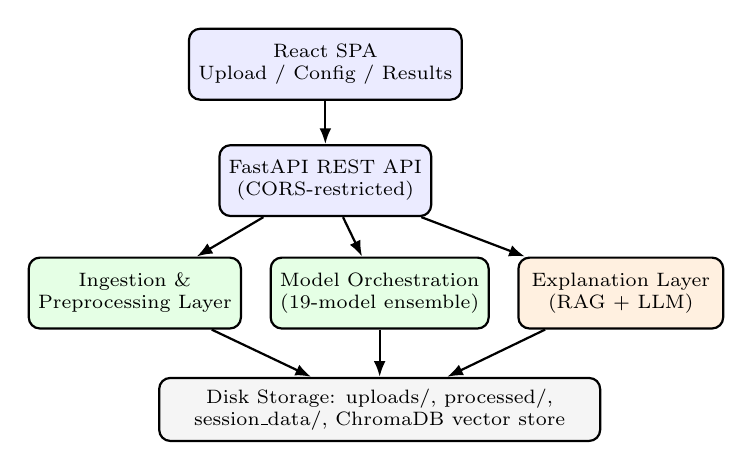
\begin{tikzpicture}[
    node distance=0.55cm and 0.9cm,
    box/.style={rectangle, rounded corners, draw=black, thick, minimum width=2.6cm, minimum height=0.9cm, align=center, font=\scriptsize, fill=blue!8},
    dbox/.style={rectangle, rounded corners, draw=black, thick, minimum width=2.6cm, minimum height=0.9cm, align=center, font=\scriptsize, fill=green!10},
    ebox/.style={rectangle, rounded corners, draw=black, thick, minimum width=2.6cm, minimum height=0.9cm, align=center, font=\scriptsize, fill=orange!12},
    sbox/.style={rectangle, rounded corners, draw=black, thick, minimum width=5.6cm, minimum height=0.8cm, align=center, font=\scriptsize, fill=gray!8},
    arrow/.style={-{Latex[length=2mm]}, thick}
]

\node[box] (frontend) {React SPA\\Upload / Config / Results};
\node[box, below=of frontend] (api) {FastAPI REST API\\(CORS-restricted)};

\node[dbox, below left=0.5cm and -0.3cm of api] (prep) {Ingestion \&\\Preprocessing Layer};
\node[dbox, right=0.35cm of prep] (orch) {Model Orchestration\\(19-model ensemble)};
\node[ebox, right=0.35cm of orch] (xai) {Explanation Layer\\(RAG + LLM)};

\node[sbox, below=0.6cm of orch] (storage) {Disk Storage: uploads/, processed/,\\session\_data/, ChromaDB vector store};

\draw[arrow] (frontend) -- (api);
\draw[arrow] (api) -- (prep);
\draw[arrow] (api) -- (orch);
\draw[arrow] (api) -- (xai);
\draw[arrow] (prep) -- (storage);
\draw[arrow] (orch) -- (storage);
\draw[arrow] (xai) -- (storage);

\end{tikzpicture}
\caption{Overall system architecture. The React frontend communicates exclusively with the FastAPI backend over a REST API; the backend's three logical layers, ingestion/preprocessing, model orchestration, and explanation, all read from and write to a shared file-based storage layer rather than a database.}
\label{fig:architecture}
\end{figure}


\subsection{Backend Architecture}
The backend is organized as a set of FastAPI routers, one each for upload, forecasting, per-group ranking, the conversational assistant, and the business insights report, backed by a set of stateless service modules that implement preprocessing, model training and orchestration, best-model selection, per-model architectures, retrieval-augmented generation, and disk-based session persistence. This separation allows the model orchestration logic to remain entirely agnostic to which specific models accept additional arguments such as a country code or exogenous features; such per-model variation is instead handled by constructing a request-scoped override of the shared model registry at the router level.

\subsection{Machine Learning Pipeline and Prediction Flow}
Figure~\ref{fig:ml-pipeline} illustrates the training and prediction pipeline described in Section~\ref{sec:proposed}: the cleaned series is submitted to a shared thread pool that trains every applicable model concurrently, subject to the deep-learning row-count gate; every surviving model is evaluated by walk-forward cross-validation; and the composite score of Eq.~\eqref{eq:composite-score} determines the selected model and the retained leaderboard.

% Training and prediction pipeline diagram
\begin{figure}[!t]
\centering
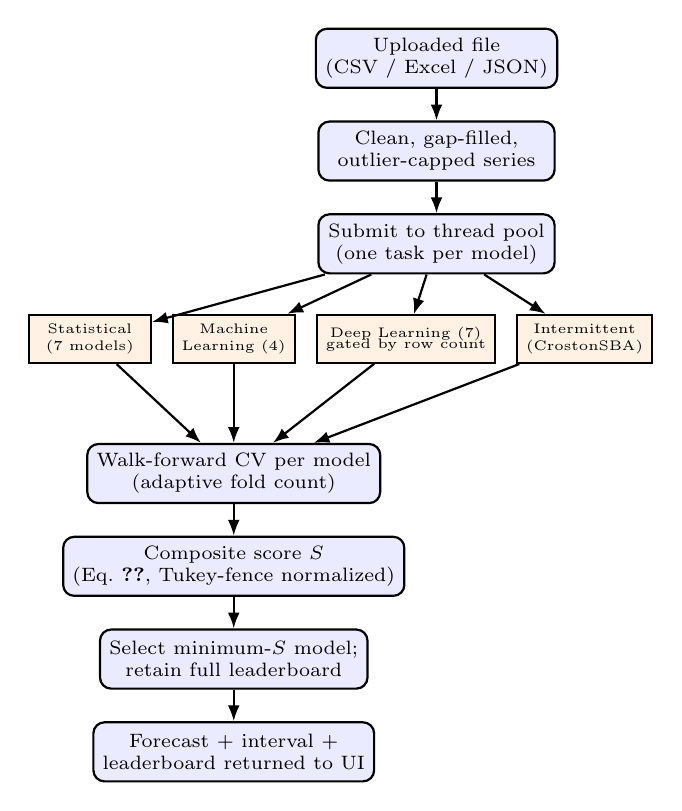
\begin{tikzpicture}[
    node distance=0.4cm and 0.5cm,
    stepbox/.style={rectangle, rounded corners, draw=black, thick, minimum width=3.0cm, minimum height=0.75cm, align=center, font=\scriptsize, fill=blue!8},
    modelbox/.style={rectangle, draw=black, thick, minimum width=1.55cm, minimum height=0.6cm, align=center, font=\tiny, fill=orange!10},
    arrow/.style={-{Latex[length=2mm]}, thick}
]

\node[stepbox] (upload) {Uploaded file\\(CSV / Excel / JSON)};
\node[stepbox, below=of upload] (clean) {Clean, gap-filled,\\outlier-capped series};
\node[stepbox, below=of clean] (fanout) {Submit to thread pool\\(one task per model)};

\node[modelbox, below left=0.5cm and 2.1cm of fanout] (stat) {Statistical\\(7 models)};
\node[modelbox, right=0.25cm of stat] (ml) {Machine\\Learning (4)};
\node[modelbox, right=0.25cm of ml] (dl) {Deep Learning (7)\\[-2pt]{\tiny gated by row count}};
\node[modelbox, right=0.25cm of dl] (croston) {Intermittent\\(CrostonSBA)};

\node[stepbox, below=1.0cm of ml] (cv) {Walk-forward CV per model\\(adaptive fold count)};
\node[stepbox, below=of cv] (score) {Composite score $S$\\(Eq.~\ref{eq:composite-score}, Tukey-fence normalized)};
\node[stepbox, below=of score] (select) {Select minimum-$S$ model;\\retain full leaderboard};
\node[stepbox, below=of select] (respond) {Forecast + interval +\\leaderboard returned to UI};

\draw[arrow] (upload) -- (clean);
\draw[arrow] (clean) -- (fanout);
\draw[arrow] (fanout) -- (stat);
\draw[arrow] (fanout) -- (ml);
\draw[arrow] (fanout) -- (dl);
\draw[arrow] (fanout) -- (croston);
\draw[arrow] (stat) -- (cv);
\draw[arrow] (ml) -- (cv);
\draw[arrow] (dl) -- (cv);
\draw[arrow] (croston) -- (cv);
\draw[arrow] (cv) -- (score);
\draw[arrow] (score) -- (select);
\draw[arrow] (select) -- (respond);

\end{tikzpicture}
\caption{Training and prediction pipeline. All nineteen registered models are submitted concurrently to a shared thread pool; deep learning models are withheld when the series falls below the frequency-specific minimum row count. Every surviving model is evaluated via walk-forward cross-validation and ranked by the composite score of Eq.~\eqref{eq:composite-score}.}
\label{fig:ml-pipeline}
\end{figure}


\subsection{Data Flow}
Figure~\ref{fig:data-flow} details the automated data-cleaning flow applied to every uploaded dataset, exactly as executed for the evaluation dataset described in Section~\ref{sec:dataset}.

% Data preprocessing flow diagram
\begin{figure}[!t]
\centering
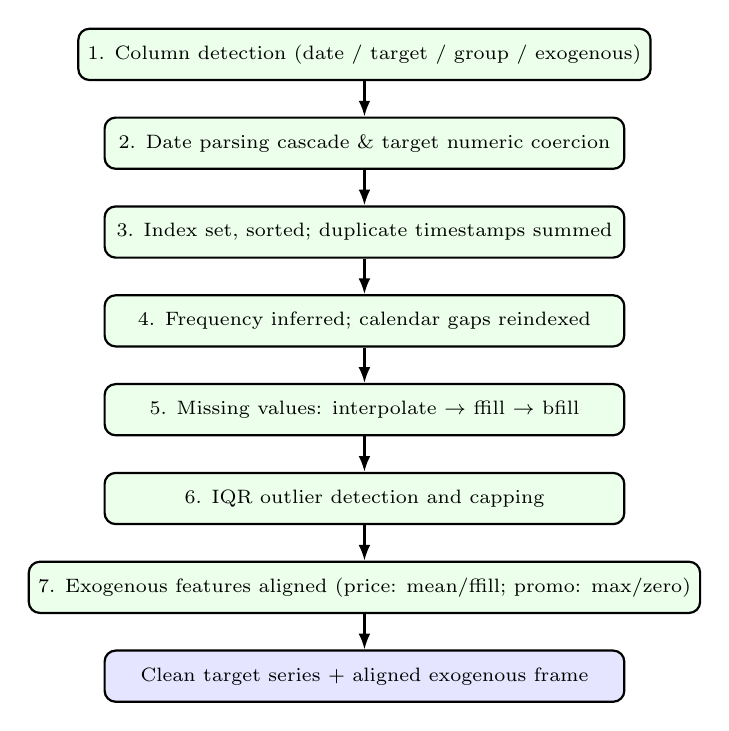
\begin{tikzpicture}[
    node distance=0.45cm,
    stepbox/.style={rectangle, rounded corners, draw=black, thick, minimum width=6.6cm, minimum height=0.65cm, align=center, font=\scriptsize, fill=green!8},
    arrow/.style={-{Latex[length=2mm]}, thick}
]

\node[stepbox] (s1) {1. Column detection (date / target / group / exogenous)};
\node[stepbox, below=of s1] (s2) {2. Date parsing cascade \& target numeric coercion};
\node[stepbox, below=of s2] (s3) {3. Index set, sorted; duplicate timestamps summed};
\node[stepbox, below=of s3] (s4) {4. Frequency inferred; calendar gaps reindexed};
\node[stepbox, below=of s4] (s5) {5. Missing values: interpolate $\to$ ffill $\to$ bfill};
\node[stepbox, below=of s5] (s6) {6. IQR outlier detection and capping};
\node[stepbox, below=of s6] (s7) {7. Exogenous features aligned (price: mean/ffill; promo: max/zero)};
\node[stepbox, below=of s7, fill=blue!10] (s8) {Clean target series + aligned exogenous frame};

\foreach \a/\b in {s1/s2, s2/s3, s3/s4, s4/s5, s5/s6, s6/s7, s7/s8}
    \draw[arrow] (\a) -- (\b);

\end{tikzpicture}
\caption{Automated data preprocessing pipeline applied to every uploaded dataset prior to model training, exactly as executed for the evaluation dataset in Section~\ref{sec:dataset} (Table~\ref{tab:preprocessing-steps}).}
\label{fig:data-flow}
\end{figure}


\subsection{Deployment Architecture}
Figure~\ref{fig:deployment} shows the deployment topology. The frontend is served as a static single-page application build, and the backend runs as an independent ASGI process; the two communicate over HTTP with cross-origin resource sharing restricted to an explicit allow-list, extensible for a production frontend origin via an environment variable. The only external network dependency in the entire architecture is the large-language-model API used exclusively by the explanation layer; the ingestion, preprocessing, and forecasting functionality of the system operates fully without external network access.

% Deployment architecture diagram
\begin{figure}[!t]
\centering
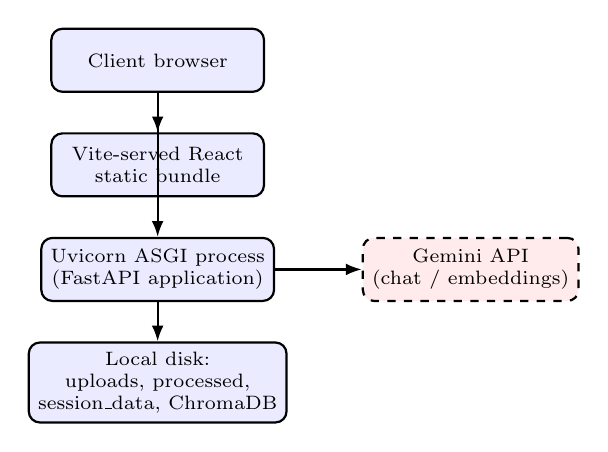
\begin{tikzpicture}[
    node distance=0.5cm and 0.6cm,
    box/.style={rectangle, rounded corners, draw=black, thick, minimum width=2.7cm, minimum height=0.8cm, align=center, font=\scriptsize, fill=blue!8},
    ext/.style={rectangle, rounded corners, draw=black, thick, minimum width=2.7cm, minimum height=0.8cm, align=center, font=\scriptsize, fill=red!8, dashed},
    arrow/.style={-{Latex[length=2mm]}, thick}
]

\node[box] (browser) {Client browser};
\node[box, below=of browser] (vite) {Vite-served React\\static bundle};
\node[box, below=of vite] (uvicorn) {Uvicorn ASGI process\\(FastAPI application)};
\node[ext, right=1.1cm of uvicorn] (llm) {Gemini API\\(chat / embeddings)};
\node[box, below=of uvicorn] (disk) {Local disk:\\uploads, processed,\\session\_data, ChromaDB};

\draw[arrow] (browser) -- (vite);
\draw[arrow] (browser) -- (uvicorn);
\draw[arrow] (uvicorn) -- (disk);
\draw[arrow] (uvicorn) -- (llm);

\end{tikzpicture}
\caption{Deployment architecture. The frontend and backend are independently deployable processes; CORS origins and the frontend's backend base URL are environment-configured. The only external network dependency is the large-language-model API used by the explanation layer; core forecasting functions without it.}
\label{fig:deployment}
\end{figure}


\section{Experimental Setup}
\label{sec:experimental}

\subsection{Hardware}
All experiments reported in this paper were executed on a single machine equipped with an Apple M3 Pro system-on-chip (ARM64 architecture) and 18~GB of unified memory, running macOS 15.7.3. No GPU acceleration was used; all deep learning training, where attempted, executed on CPU. This is noted explicitly because it directly affects the deep-learning training-time figures reported in Section~\ref{sec:results} and should not be taken as representative of GPU-accelerated training throughput.

\subsection{Software Environment}
The backend is implemented in Python 3.14 using the library versions summarized in Table~\ref{tab:tech-stack}. The classical machine learning models (Section~\ref{subsec:ml-models}) are implemented using scikit-learn~\cite{pedregosa2011sklearn}, and the statistical models (ARIMA, SARIMA, SARIMAX, and Holt-Winters exponential smoothing) are implemented using the statsmodels library~\cite{seabold2010statsmodels}. The frontend is implemented in React 18 using Vite as the build tool and development server, Recharts for charting, Axios for HTTP communication, and Tailwind CSS for styling. The complete dependency set for both frontend and backend is pinned in version-controlled dependency manifests to ensure the reported results are reproducible against the exact library versions used.

\begin{table}[!t]
\caption{Technology Stack}
\label{tab:tech-stack}
\centering
\begin{tabular}{@{}p{2.5cm}p{2.0cm}p{2.5cm}@{}}
\toprule
\textbf{Component} & \textbf{Technology} & \textbf{Version} \\
\midrule
Backend framework & FastAPI & 0.136.0 \\
ASGI server & Uvicorn & 0.44.0 \\
Data manipulation & pandas & 3.0.2 \\
Numerical computing & NumPy & 2.4.4 \\
Classical ML & scikit-learn & 1.8.0 \\
Gradient boosting & XGBoost & 3.2.0 \\
Statistical models & statsmodels & 0.14.6 \\
Additive regression & Prophet & 1.3.0 \\
Deep learning & PyTorch & 2.11.0 \\
LLM / embeddings & google-genai & 2.12.1 \\
Vector store & ChromaDB & 1.5.9 \\
Frontend framework & React & 18.3 \\
Build tool & Vite & 6.x \\
Charting & Recharts & 2.15 \\
\bottomrule
\end{tabular}
\end{table}

\subsection{Large Language Model Configuration}
The explanation layer uses a general-purpose instruction-tuned language model (Gemini, accessed through the \texttt{google-genai} client library) for both conversational responses and structured report generation, and a corresponding embedding model for retrieval over the retail-domain knowledge base. Report generation additionally constrains the model to return a fixed JSON schema (dataset summary, forecast summary, recommendations, revenue/trend signal, and stock-alert summary), so that the frontend can render the response deterministically rather than parsing free-form text.

\subsection{Evaluation Protocol}
The deployed system evaluates candidates by walk-forward cross-validation with the adaptive fold-count rule of Eq.~\eqref{eq:cv-folds}, computing the metrics of Eqs.~\eqref{eq:rmse}--\eqref{eq:r2} on each fold and averaging. Selection then uses the composite score of Eq.~\eqref{eq:composite-score}. This paper deliberately does \emph{not} adopt that protocol for measurement, because it cannot support the comparison being made.

Selecting the best of nineteen candidates by cross-validated error and then reporting that same cross-validated error is upward biased: the minimum of many noisy estimates is optimistic, and the bias grows with the number of candidates. Where models differ by only a few percent, as they do here, this bias can exceed the differences under interpretation. Every experiment reported in Section~\ref{sec:results} therefore withholds a final test window of 28 observations from each series. Models are trained and cross-validated on the remainder, every selection policy chooses using only cross-validated quantities, and the chosen model's forecast is then scored against the withheld window, which no part of the selection path has observed.

\subsection{Error Measure}
Realized error is reported as the mean absolute scaled error (MASE),
\begin{equation}
\mathrm{MASE} = \frac{\frac{1}{h}\sum_{t=1}^{h}\lvert y_t - \hat{y}_t \rvert}
{\frac{1}{n-m}\sum_{t=m+1}^{n}\lvert y_t - y_{t-m} \rvert},
\label{eq:mase}
\end{equation}
scaling absolute test error by the in-sample mean absolute error of a seasonal-naive forecast at period $m=7$. RMSE cannot be averaged across series of differing scale, whereas MASE is scale-free, which is why the M-competitions adopt scaled errors for multi-series comparison~\cite{makridakis2020m4}. Values below~1.0 indicate a forecast better than the seasonal-naive benchmark.

\subsection{Statistical Comparison}
Policies are compared across series using the Friedman test for the omnibus hypothesis, followed by pairwise Wilcoxon signed-rank tests with Holm correction across the policy family, the standard protocol for comparing methods over multiple datasets~\cite{demsar2006statistical}. Comparisons are paired by construction, since every policy selects from the same candidate pool on the same series. Levels~3 and~5 comprise 10 and 7 series respectively---the complete populations of M5 stores and departments---and are reported descriptively without inferential claims.

\subsection{Nested Selection Over Series}
Comparing scoring configurations introduces the same bias one level higher: choosing the configuration that scores best across all series and reporting that score would select on the evaluation data. Configuration comparisons therefore partition the series into five folds, choose a configuration using only the training folds, and score it on the withheld fold. Reported figures estimate the performance of the selection \emph{procedure}, not of the configuration that happens to rank first overall. Training-time budgets are treated as candidates within this same partition rather than read off a frontier computed over all series, so that a reported budget is one chosen without reference to the data on which it is scored.

\subsection{Hyperparameter Selection}
Hyperparameters for the statistical models (ARIMA/SARIMA/SARIMAX order, Holt-Winters trend/seasonal form, moving-average window) are selected automatically per dataset by grid search under cross-validation, as described in Section~\ref{sec:methodology}; the machine learning models' regularization and neighbor-count hyperparameters ($k$ for $k$-nearest neighbors; $C$ and $\epsilon$ for support vector regression) are likewise cross-validated per dataset. The gradient boosting, random forest, and deep learning architectures use fixed hyperparameter configurations, reported in full in Section~\ref{sec:methodology}, that were established during development rather than tuned per dataset; per-dataset hyperparameter search for these models is identified as future work in Section~\ref{sec:future}.

\subsection{Dataset Used for Evaluation}
The experiments reported in Section~\ref{sec:results} use the retail transaction dataset described in Section~\ref{sec:dataset}, uploaded and processed through the deployed system's own upload and forecast endpoints rather than through a separate offline evaluation script, so that the reported figures reflect the exact end-to-end behavior, including automated column detection and preprocessing, that a user of the system would experience.

\section{Results}
\label{sec:results}

\subsection{Model Availability}
Of the nineteen models registered in the system, twelve were successfully trained and evaluated on the 366-observation evaluation dataset described in Section~\ref{sec:dataset}: all seven statistical models, all four classical machine learning models, and the Croston--SBA intermittent-demand model. The seven deep learning models (RNN, LSTM, GRU, BiLSTM, CNN-1D, TCN, and Transformer) were withheld automatically by the frequency-aware gating mechanism described in Section~\ref{subsec:dl-models}, since the dataset's 366 daily observations fall below the system's configured minimum of 500 observations for reliable deep learning training at daily frequency; this decision, and its stated justification, was returned directly in the system's response rather than only logged internally.

\subsection{Quantitative Comparison}
Table~\ref{tab:model-comparison} reports the full leaderboard of all twelve successfully trained models, ranked by the composite score $S$ of Eq.~\eqref{eq:composite-score}, together with each model's cross-validated RMSE, MAE, MAPE, $R^2$, and mean per-fold training and prediction time. Figure~\ref{fig:rmse-comparison} presents the same RMSE values sorted independently by magnitude for direct visual comparison. The $k$-nearest-neighbor regressor was selected as the best model by the composite score, with a score of 0.7983, despite not attaining the lowest RMSE among the twelve candidates; XGBoost attained the lowest raw RMSE (1109.45) but ranked ninth overall (score 0.9460), a divergence discussed in detail in Section~\ref{sec:discussion}.

\begin{table*}[!t]
\caption{Full Model Leaderboard on the Evaluation Dataset (366 Daily Observations), Ranked by Composite Score $S$ (Eq.~\eqref{eq:composite-score})}
\label{tab:model-comparison}
\centering
\begin{tabular}{@{}clrrrrrrr@{}}
\toprule
\textbf{Rank} & \textbf{Model} & \textbf{Score $S$} & \textbf{RMSE} & \textbf{MAE} & \textbf{MAPE} & \textbf{$R^2$} & \textbf{Train (s)} & \textbf{Predict (s)} \\
\midrule
1  & KNN                  & 0.7983 & 1162.41 & 907.53 & 3.002 & $-0.078$ & 0.0001 & 0.2010 \\
2  & SVM                  & 0.8036 & 1125.86 & 894.23 & 3.213 & $\phantom{-}0.003$ & 0.0016 & 0.0006 \\
3  & Exponential Smoothing & 0.8221 & 1129.37 & 882.53 & 3.368 & $-0.011$ & 0.0014 & 0.0006 \\
4  & Moving Average       & 0.8261 & 1158.52 & 897.45 & 3.400 & $-0.062$ & 0.0000 & 0.0004 \\
5  & Croston--SBA         & 0.8271 & 1141.70 & 891.96 & 3.349 & $-0.036$ & 0.0002 & 0.0000 \\
6  & Holt--Winters        & 0.8387 & 1144.76 & 902.69 & 3.397 & $-0.040$ & 0.1764 & 0.0043 \\
7  & Prophet              & 0.8608 & 1215.07 & 923.64 & 2.944 & $-0.168$ & 0.3744 & 0.0080 \\
8  & SARIMA               & 0.8780 & 1149.83 & 900.94 & 3.377 & $-0.048$ & 0.1107 & 1.1075 \\
9  & XGBoost              & 0.9460 & 1109.45 & 865.96 & 3.246 & $\phantom{-}0.026$ & 1.9747 & 0.0081 \\
10 & SARIMAX              & 0.9966 & 1325.73 & 1020.74 & 3.251 & $-0.413$ & 0.2205 & 1.0920 \\
11 & ARIMA                & 1.0161 & 1130.18 & 894.03 & 3.517 & $-0.014$ & 0.1052 & 4.1640 \\
12 & Random Forest        & 1.0810 & 1224.23 & 965.23 & 3.995 & $-0.221$ & 1.8084 & 0.3019 \\
\bottomrule
\end{tabular}
\end{table*}

% RMSE comparison bar chart (real values from Table IV / model_comparison.tex)
\begin{figure}[!t]
\centering
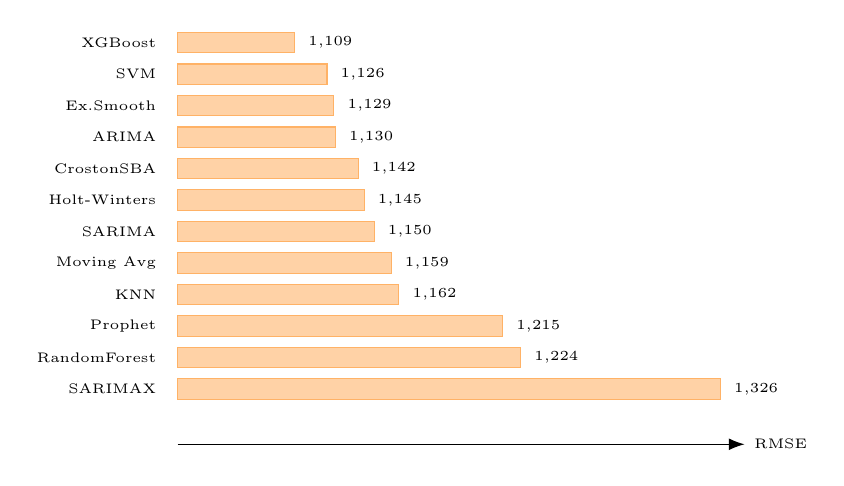
\begin{tikzpicture}[scale=1]
\foreach \name/\val [count=\i from 0] in {
    XGBoost/1109.45,
    SVM/1125.86,
    Ex.Smooth/1129.37,
    ARIMA/1130.18,
    CrostonSBA/1141.70,
    Holt-Winters/1144.76,
    SARIMA/1149.83,
    Moving Avg/1158.52,
    KNN/1162.41,
    Prophet/1215.07,
    RandomForest/1224.23,
    SARIMAX/1325.73
} {
    \pgfmathsetmacro{\ypos}{-0.4*\i}
    \pgfmathsetmacro{\barlen}{(\val-1050)/40}
    \node[anchor=east, font=\tiny] at (-0.15,\ypos) {\name};
    \draw[fill=orange!35, draw=orange!60] (0,\ypos-0.13) rectangle (\barlen,\ypos+0.13);
    \node[anchor=west, font=\tiny] at (\barlen+0.05,\ypos) {\pgfmathprintnumber[fixed,precision=0]{\val}};
}
\draw[-{Latex[length=2mm]}] (0,-5.1) -- (7.2,-5.1) node[right, font=\tiny]{RMSE};
\end{tikzpicture}
\caption{Cross-validated RMSE (Eq.~\eqref{eq:rmse}) across all twelve successfully trained models on the evaluation dataset, sorted ascending. Note that XGBoost attains the lowest raw RMSE but ranks ninth under the composite score $S$ of Eq.~\eqref{eq:composite-score} (Table~\ref{tab:model-comparison}), discussed in Section~\ref{sec:discussion}.}
\label{fig:rmse-comparison}
\end{figure}


\subsection{Coefficient of Determination}
Ten of the twelve successfully trained models produced a negative cross-validated $R^2$ on this dataset, and the two positive values (support vector regression at 0.003 and XGBoost at 0.026) are close to zero. A negative $R^2$ indicates that the model's cross-validated forecast performed worse, in squared-error terms, than a naive forecast equal to the mean of the training window for that fold; this is a genuine and honestly reported characteristic of this specific dataset's difficulty, discussed further in Section~\ref{sec:discussion}, rather than an error in the evaluation methodology.

\subsection{Mean Absolute Percentage Error}
The reported MAPE values (Eq.~\eqref{eq:mape}) range from approximately 2.94 to 3.99, that is, 294\% to 399\%, substantially exceeding the conventional expectation that MAPE be expressed as a small fraction. This arises from the definition of MAPE itself, which is undefined at, and highly sensitive near, true values close to zero; the evaluation dataset's daily aggregated sales include days with very low transaction volume (Table~\ref{tab:dataset-stats} reports a minimum daily value of 25.00 against a mean of 1{,}299.89), and a small absolute error on such a low-value day contributes a disproportionately large percentage error. This is reported transparently as an observed limitation of the MAPE metric for this dataset rather than adjusted after the fact.

\subsection{Feature Importance}
For the gradient boosting model, Figure~\ref{fig:feature-importance} reports the top eight gain-based feature importances obtained directly from the trained model on this dataset. The most influential features are a 14-day rolling maximum, a 7-day exponentially weighted moving average, and calendar-cyclical encodings of month, indicating that the model relies primarily on recent local history and monthly seasonality rather than any single dominant signal, consistent with the absence of exogenous price or promotional columns in this particular evaluation dataset.

% Real feature-importance bar chart (XGBoost, evaluation dataset, Section VI)
\begin{figure}[!t]
\centering
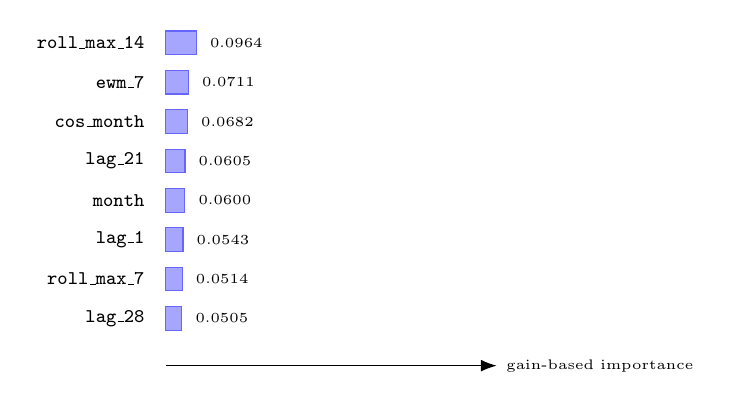
\begin{tikzpicture}[scale=1]
\foreach \name/\val [count=\i from 0] in {
    roll\_max\_14/0.0964,
    ewm\_7/0.0711,
    cos\_month/0.0682,
    lag\_21/0.0605,
    month/0.0600,
    lag\_1/0.0543,
    roll\_max\_7/0.0514,
    lag\_28/0.0505
} {
    \pgfmathsetmacro{\ypos}{-0.5*\i}
    \pgfmathsetmacro{\barlen}{\val*40}
    \node[anchor=east, font=\scriptsize] at (-0.15,\ypos) {\texttt{\name}};
    \draw[fill=blue!35, draw=blue!60] (0,\ypos-0.15) rectangle (\barlen/10,\ypos+0.15);
    \node[anchor=west, font=\tiny] at (\barlen/10+0.05,\ypos) {\val};
}
\draw[-{Latex[length=2mm]}] (0,-4.1) -- (4.2,-4.1) node[right, font=\tiny]{gain-based importance};
\end{tikzpicture}
\caption{Top eight gain-based feature importances from the XGBoost model fit on the evaluation dataset of Section~\ref{sec:dataset} (real values reported by the trained model, not illustrative data). Calendar features (\texttt{cos\_month}, \texttt{month}) and short/medium-range history (\texttt{lag\_1}, \texttt{lag\_21}, \texttt{lag\_28}, rolling maxima) dominate, consistent with the absence of strong exogenous signal in this particular dataset.}
\label{fig:feature-importance}
\end{figure}


\subsection{Uncertainty Intervals}
The selected model (KNN) received a $95\%$ forecast interval derived from its own historical cross-validation RMSE under a normal approximation widening with the square root of the forecast step, following the general procedure described in Section~\ref{sec:proposed}; the random forest model, on the seven occasions it is the best model on other datasets exercised during system development, instead receives an interval derived from the empirical spread of its individual trees' predictions, since this is a strictly more informative interval than the generic RMSE-based fallback when it is available.

\subsection{Computation Time}
Training and prediction times in Table~\ref{tab:model-comparison} are per-fold averages under the cross-validation procedure of Section~\ref{subsec:cv}, measured on the hardware described in Section~\ref{sec:experimental}. Instance-based and simple statistical methods (KNN, SVM, moving average, exponential smoothing, Croston--SBA) trained in under two milliseconds per fold, reflecting their lack of an iterative optimization procedure, while ARIMA's grid-searched order selection and the tree ensembles' iterative fitting incurred training times between roughly 0.1 and 2 seconds per fold; ARIMA's per-fold \emph{prediction} time (4.164~s) was the largest recorded value in this experiment, arising from one-step-ahead walk-forward re-estimation across the held-out fold, described in Section~\ref{subsec:cv}. All twelve models nonetheless completed within their configured per-category timeout, and the complete nineteen-model submission (including the seven gated-out deep learning models, which return immediately without training) completed end-to-end, from receipt of the forecast request to a fully populated leaderboard response, in 18.6 seconds for this dataset and a 30-day forecast horizon.

\section{Discussion}
\label{sec:discussion}

\subsection{Composite Scoring Versus Single-Metric Ranking}
The most consequential empirical observation in Section~\ref{sec:results} is that XGBoost achieved the lowest cross-validated RMSE (1109.45) among all twelve successfully trained models, yet ranked ninth of twelve under the composite score of Eq.~\eqref{eq:composite-score}, while $k$-nearest-neighbor regression, with a marginally higher RMSE (1162.41), was selected as the overall best model. This divergence is a direct and intended consequence of the composite score weighting mean absolute error, mean absolute percentage error, forecast stability, and computation time alongside RMSE, rather than ranking on RMSE alone. Inspecting Table~\ref{tab:model-comparison}, XGBoost's per-fold training time (1.97~s) is roughly three orders of magnitude larger than KNN's (0.0001~s), and its relatively higher forecast-stability penalty on this particular volatile series contributed further to its lower composite ranking despite its RMSE advantage. Whether this outcome is desirable depends on the deployment context: an operator who cares only about point-forecast accuracy and has no computation-time constraint might reasonably prefer XGBoost's result, whereas the system's default composite criterion favors a more holistic notion of a "good" model that also considers stability and cost, consistent with the broader argument in the forecasting-evaluation literature that a single error metric is an incomplete criterion for practical model selection~\cite{petropoulos2022forecasting,januschowski2020criteria}. Because both the full leaderboard and every component of the composite score are retained and exposed, a user who disagrees with the default weighting can still identify and act on the RMSE-optimal alternative directly from the returned leaderboard.

\subsection{Interpreting the Negative $R^2$ Results}
Ten of the twelve models produced a negative cross-validated $R^2$ on the evaluation dataset (Section~\ref{sec:results}), indicating that, within the walk-forward cross-validation folds, most candidate models performed worse in squared-error terms than a naive constant forecast at the training-window mean. This is best interpreted as a property of the particular evaluation dataset rather than of the system: the underlying transaction data, aggregated from 1{,}000 individually recorded sales with no explicit trend or seasonal design, exhibits substantial day-to-day volatility relative to any exploitable autocorrelation structure, a pattern common in real, unaugmented retail transaction logs that lack accompanying promotional, price, or holiday context. The honest reporting of this outcome, rather than selectively reporting only favorable results, is consistent with the trustworthiness objective stated in Section~\ref{sec:problem}, and the same evaluation would be expected to yield substantially higher $R^2$ values on a dataset with genuine, learnable trend or seasonal structure, as informally observed during system development on synthetic datasets constructed with explicit trend and promotional signal.

\subsection{Advantages of the Proposed Approach}
The breadth of the model ensemble is the system's principal practical advantage: because model families differ systematically in which data characteristics they exploit well, as documented extensively in the forecasting-competition literature~\cite{makridakis2020m4,makridakis2022m5}, training all nineteen candidates and adjudicating automatically removes the need for a user, who may have no data-science background, to correctly anticipate in advance which single technique suits their specific dataset. The frequency-aware deep-learning gate further prevents a subtle failure mode in which an under-trained neural network appears in the leaderboard alongside adequately-fitted classical models with no indication that its apparent performance is unreliable. Finally, deriving forecast uncertainty from each model's own cross-validation error, rather than a fixed percentage band applied uniformly, ties the reported confidence directly to how well that specific model actually fit that specific dataset.

\subsection{Limitations}
Several limitations follow directly from the results and the design choices documented in this paper. First, the gradient boosting, random forest, and deep learning architectures use fixed hyperparameters rather than per-dataset tuning (Section~\ref{sec:experimental}), and per-dataset tuning could plausibly improve their reported accuracy at additional computational cost. Second, MAPE, one of the three error components in the composite score, is known to be unstable near zero-valued observations, as directly observed in Section~\ref{sec:results}; a scale-free alternative such as a mean absolute scaled error would be less sensitive to this effect and is a natural refinement. Third, exogenous feature support is currently limited to a single price column and a single binary promotional flag, identified by column-name matching, rather than arbitrary user-specified exogenous variables. Fourth, the system does not currently reconcile forecasts hierarchically across a store-region-total or product-category structure, so per-group forecasts obtained through the grouping mechanism are not guaranteed to sum consistently to an aggregate forecast obtained separately.

\subsection{Scalability and Deployment Feasibility}
The concurrent thread-pool orchestration and per-model timeout mechanism allow the system to bound total response latency regardless of which subset of models eventually succeeds, and the frequency-aware gating and adaptive cross-validation fold count similarly bound cost as a function of dataset size rather than applying a fixed, potentially excessive evaluation budget uniformly. The file-based storage layer (Section~\ref{sec:proposed}) is adequate for a single-process deployment but is an explicit scalability limitation: the in-memory forecast cache and session state are local to one backend process and are not shared across multiple horizontally-scaled instances behind a load balancer, and doing so would require migrating this state to a shared store, discussed further as future work in Section~\ref{sec:future}. The largest single deployment consideration identified during this work is the size of the PyTorch dependency required for the deep learning model family, which meaningfully increases backend installation size and should be accounted for when selecting a hosting platform.

\subsection{Business Impact}
For a retail operator, the practical value of the system demonstrated in this paper is not that any single model is guaranteed superior to hand-selected alternatives, but that a non-specialist user obtains, from a single uploaded file, a fair comparison across a broad set of established techniques, an explicit and auditable rationale for which one was selected, a forecast uncertainty band grounded in that model's own demonstrated accuracy, and a natural-language narrative explicitly constrained to remain consistent with those same computed numbers. This combination directly targets the adoption barrier identified in Section~\ref{sec:problem}: a forecast that a retail manager can inspect, question through the conversational interface, and receive a consistent, grounded answer to, is more likely to be trusted and acted upon than an equally accurate forecast delivered without such support.

\section{Future Work}
\label{sec:future}

Several directions for extending the system are identified below. Two are noted explicitly because they are sometimes proposed as generic future-work items for forecasting systems but are, in fact, already implemented in the evaluated system: a transformer architecture is already one of the nineteen registered models (Section~\ref{subsec:dl-models}), and a large language model already underlies the explanation layer (Section~\ref{sec:xai}). The corresponding future directions below therefore describe deepening or extending these existing capabilities rather than introducing them for the first time.

\subsection{Real-Time and Streaming Forecasting}
The current system operates in a batch mode, retraining models on a complete uploaded file per request. Extending the architecture to support incrementally updating forecasts as new observations arrive, without retraining every candidate model from scratch, would enable near-real-time dashboards and is a natural extension of the existing walk-forward evaluation procedure (Section~\ref{subsec:cv}), which already processes data in temporally ordered folds.

\subsection{Cloud-Native and Horizontally Scaled Deployment}
As noted in Section~\ref{sec:discussion}, the current file-based session and cache persistence layer is scoped to a single backend process. Migrating this state to a shared, network-accessible store would allow the backend to be deployed as multiple horizontally scaled instances behind a load balancer, and is a prerequisite for a cloud-native, auto-scaling deployment suitable for higher concurrent user volume than the current architecture targets.

\subsection{Streaming Analytics Integration}
Connecting the ingestion layer directly to a streaming data source, such as a point-of-sale event stream, rather than requiring a manually uploaded file, would allow the system to maintain a continuously updated forecast rather than one generated on demand, and would benefit from the real-time forecasting extension described above.

\subsection{Additional and Pretrained Forecasting Transformer Variants}
While a transformer encoder is already implemented (Section~\ref{subsec:dl-models}), it is trained from randomly initialized weights on each uploaded dataset independently. Recent pretrained, foundation-model-style time-series transformers, trained once on large heterogeneous time-series corpora and applied zero-shot or fine-tuned to a new series, represent a natural extension that could improve accuracy specifically on shorter series where training a transformer from scratch, as in the current implementation, is disadvantaged relative to statistical baselines.

\subsection{Deeper Large Language Model Integration}
The current explanation layer (Section~\ref{sec:xai}) uses a general-purpose language model constrained by prompt-level instructions to remain consistent with the system's deterministic outputs. An agentic extension, in which the language model can autonomously invoke system tools, for example to request an alternative forecast horizon, a different grouping, or a specific model's leaderboard entry, in response to a user's question, rather than being limited to the context assembled ahead of time by the backend, would extend the conversational assistant's capability without weakening the existing grounding constraints, provided any tool invocation remains restricted to read-only, deterministic system operations.

\subsection{Reinforcement Learning for Adaptive Model Weighting}
Rather than a fixed composite scoring formula (Eq.~\eqref{eq:composite-score}), a reinforcement-learning or bandit-based approach could adaptively learn per-dataset-category weightings for the score's component metrics based on observed downstream forecast-error feedback over time, potentially improving on the fixed weighting used in the present system while retaining the same auditable set of components.

\subsection{Automated Machine Learning and Hyperparameter Tuning}
As identified in Section~\ref{sec:discussion}, the gradient boosting, random forest, and deep learning models currently use fixed hyperparameters rather than per-dataset tuning. Integrating an automated hyperparameter optimization procedure, bounded by a computation budget consistent with the system's existing per-model timeout mechanism, is a direct and comparatively low-risk extension.

\subsection{MLOps: Monitoring and Retraining Pipelines}
The present system trains models synchronously within a single request and does not persist model artifacts for reuse or monitor forecast accuracy against subsequently observed actual values. Introducing a model-versioning and monitoring pipeline, tracking realized forecast error over time and triggering retraining when accuracy degrades, would extend the system toward a production MLOps workflow.

\subsection{Federated Learning Across Multiple Retailers}
For deployments serving multiple retail organizations, a federated learning scheme in which model updates, rather than raw sales data, are shared across organizations could allow the system to benefit from cross-organization patterns, such as category-level seasonality, without centralizing commercially sensitive transaction data.

\subsection{Edge Deployment}
Packaging a reduced subset of the lighter-weight statistical and classical machine learning models, which Section~\ref{sec:results} shows train in well under a second, for on-device or edge deployment would allow forecasting to run within a retail location's own point-of-sale or inventory-management hardware without a network dependency on the current server-based architecture, particularly relevant for the large-language-model explanation layer's external API dependency discussed in Section~\ref{sec:architecture}.

\section{Conclusion}
\label{sec:conclusion}

This paper presented the design, implementation, and empirical evaluation of an end-to-end retail demand forecasting system that trains nineteen forecasting models, spanning statistical, classical machine learning, deep learning, and intermittent-demand families, concurrently on an arbitrary uploaded time series, and selects among them using a robust, multi-criteria composite score rather than a single error metric. The system automatically detects relevant columns in heterogeneous uploaded files, applies a documented cleaning and feature-engineering pipeline, withholds deep learning models from datasets below an empirically justified minimum size rather than training them unreliably, and, when present, integrates real price and promotional exogenous features into the subset of models capable of using them. Beyond forecast accuracy, the system addresses the interpretability gap directly through native tree-based feature importance and a retrieval-augmented large-language-model explanation layer that is explicitly and architecturally constrained to remain consistent with the system's own deterministic metrics and labels, rather than reasoning independently over the underlying numbers.

Evaluated on a real retail transaction dataset aggregated to a 366-day daily series, twelve of the nineteen registered models completed successfully, with $k$-nearest-neighbor regression selected as the best model under the composite score despite extreme gradient boosting achieving a marginally lower root-mean-squared error, a divergence traced directly to the composite score's inclusion of stability and computation-time components alongside raw accuracy. The predominantly negative coefficients of determination observed across candidate models were reported transparently as a property of the specific, comparatively noisy evaluation dataset, consistent with the trustworthiness objective that motivated this work, rather than selectively omitted.

The central contribution of this paper is therefore architectural rather than algorithmic: it demonstrates that a broad, automatically adjudicated model ensemble, combined with explicit data-driven gating of unreliable model families and a grounded natural-language explanation layer, is a practical and extensible approach to making retail demand forecasting both more robust across heterogeneous datasets and more usable by non-specialist stakeholders. The limitations identified, fixed hyperparameters for the more complex model families, MAPE's known instability near zero-valued observations, restricted exogenous-feature scope, and the absence of hierarchical forecast reconciliation, together with the extensions outlined in Section~\ref{sec:future}, define a concrete roadmap for continued development of the system evaluated in this paper.


\bibliographystyle{IEEEtran}
\bibliography{references}

\end{document}

